\documentclass{report}

\usepackage{amsthm,amsmath,amssymb,amsfonts,amscd}
\usepackage{graphicx}
\usepackage{enumerate}
\usepackage[all]{xy}
\usepackage{booktabs}
\usepackage{todonotes}
\usepackage{algorithm2e}
\usepackage{tikz-network}
\usepackage{caption}
\usepackage{subcaption}

\RestyleAlgo{ruled}




\newtheorem{theorem}{Theorem}[section]
\newtheorem{lemma}[theorem]{Lemma}
\newtheorem{proposition}[theorem]{Proposition}
\newtheorem{observation}[theorem]{Observation}
\newtheorem{conjecture}[theorem]{Conjecture}


\theoremstyle{definition}
\newtheorem{definition}[theorem]{Definition}
\newtheorem{example}[theorem]{Example}

\newcommand{\gobblecode}[1]{}

\newcommand{\VertexI}[2][]{\Vertex[#1, color=black, shape=circle, size=0.25]{#2}}
\newcommand{\VertexII}[2][]{\Vertex[#1, color=white, shape=semicircle, size=0.25]{#2}}
\newcommand{\VertexIII}[2][]{\Vertex[#1, color=white, style={regular polygon, regular polygon sides=3}]{#2}}
\newcommand{\VertexIV}[2][]{\Vertex[#1, color=white, style={regular polygon, regular polygon sides=4}]{#2}}
\newcommand{\VertexV}[2][]{\Vertex[#1, color=white, style={regular polygon, regular polygon sides=5}]{#2}}
\newcommand{\VertexInv}[2][]{\Vertex[#1, color=white, shape=circle, size=-1.0, style={opacity=0.0}, Pseudo=true]{#2}}


\usepackage[backend=bibtex]{biblatex}

\bibliography{references.bib}

\begin{document}

\begin{titlepage}
    \begin{center}
        \vspace*{1cm}
            
        \Huge
        \textbf{A Computational Approach for Finding 6-List-Critical Graphs on the Torus}
            
        \vspace{0.5cm}
        \Large
        \textit{Félix Moreno Peñarrubia}
            
        
            
        \,Treball de Final de Grau
            
        \vspace{0.8cm}
            
       
            
        \Large
        Grau en Matemàtiques, FME-UPC \\
        Grau en Enginyeria Informàtica, FIB-UPC \\
        \vspace{1.2cm}
        
        \includegraphics[height=1.1cm]{figures/logo_CFIS.jpg}
          \\
        
\includegraphics[height=0.8cm]{figures/logo_FME_cropped.png}
        
\includegraphics[height=0.8cm]{figures/logo_FIB.jpg}
        \\
        
\includegraphics[height=2.5cm]{figures/logo_MFF.png}
        \vfill
        
      
        May 2023
        
		\vspace{2cm}
		\large        
        \textit{Director: Zdeněk Dvořák \hspace{3cm} Tutor: Oriol Serra Albó}
        
        
            
    \end{center}
\end{titlepage}

\listoftodos

\newpage

\section*{Abstract}

Coloring graphs embedded on surfaces is an old and well-studied area of graph theory. Thomassen proved that there are finitely many $6$-critical graphs on any fixed surface and provided the explicit set of $6$-critical graphs on the torus. Later, Postle proved that there are finitely many $6$-list-critical graphs on any fixed surface. With the goal of finding the set of $6$-list-critical graphs on the torus, we develop and implement algorithmic techniques for computer search of critical graphs in different list-coloring settings. 

\textbf{Keywords:} graphs on surfaces, list coloring, graph algorithms.

\textbf{MSC2020 codes:} 05C10, 05C15, 68R10.

\section*{Resum}

La coloració de grafs dibuixats a superfícies és un àrea antiga i molt estudiada de la teoria de grafs. Thomassen va demostrar que hi ha un nombre finit de grafs $6$-crítics a qualsevol superfície fixa i va proporcionar el conjunt explícit dels grafs $6$-crítics al torus. Després, Postle va demostrar que hi ha un nombre finit de grafs $6$-llista-crítics a qualsevol superfície fixa. Amb l'objectiu de trobar el conjunt de grafs $6$-llista-crítics al torus, desenvolupem i implementem tècniques algorítmiques per la cerca per ordinador de grafs crítics en diferents situacions de coloració per llistes.  

\textbf{Paraules clau:} grafs en superfícies, coloració amb llistes, algorismes sobre grafs.

\textbf{Codis MSC2020:} 05C10, 05C15, 68R10.


\section*{Resumen}

La coloración de grafos dibujados en superficies es un área antigua y muy estudiada de la teoría de grafos. Thomassen demostró que hay un número finito de grafos $6$-críticos en cualquier superficie fija y proporcionó el conjunto explícit de los grafos $6$-críticos en el toro. Después, Postle demostró que hay un número finito de grafos 6-lista-críticos en cualquier superficie fija. Con el objetivo de encontrar el conjunto de grafos $6$-lista-críticos en el toro, desarrollamos e implementamos técnicas algorítmicas para la búsqueda por ordenador de grafos críticos en diferentes situaciones de coloración por listas.

\textbf{Palabras clave:} grafos en superficies, coloración con listas, algoritmos sobre grafos.

\textbf{Códigos MSC2020:} 05C10, 05C15, 68R10.

\newpage

\tableofcontents

\newpage

\todo{fix function restrictions}

\chapter{Introduction}

In this chapter, we lay out the basic definitions of graph theoretical and topological concepts used in this thesis, as well as the background results which contextualize our research.

We follow the exposition of Diestel \cite{diestel}, of Mohar and Thomassen \cite{graphsonsurfaces}
and of Postle \cite{postlethesis}. 

\section{Graphs and Surfaces}


\subsection{Graph Theory Terminology}

\begin{definition}
A \emph{graph} $G$ is a pair $(V(G), E(G))$ consisting of a set $V(G)$ and a set $E(G)$ of two-
element subsets of $V(G)$. We call the elements of $V(G)$ vertices and
the elements $\{u, v\}$ of $E(G)$ edges, which we often denote as $uv$.
\end{definition}



\todo{(connectivity, complete graphs, etc)}

\subsection{Surfaces}

\begin{definition}
A \emph{surface} is a connected compact $2$-dimensional manifold without boundary. 
\end{definition}

\begin{example}
The \emph{sphere} $S_0$ is the surface defined by the set $\{(x, y, z) \in \mathbb{R}^3 : x^2+y^2
+z^2 = 1\}$ with the euclidean metric inherited from $\mathbb{R}^3$. 

The \emph{torus} $S_1$ is the surface defined by the set $\{(x, y, z) \in \mathbb{R}^3 :  (\sqrt{x^2 + y^2} - 2)^2 + z^2 = 1\}$ with the euclidean metric inherited from $\mathbb{R}^3$.
\end{example}

Note that, even though we have defined the above example surfaces as geometric objects in
$\mathbb{R}^3$, we think of surfaces as \emph{topological} objects, and therefore consider two
surfaces equivalent if they are \emph{homeomorphic}. 

An important result in topology is that all surfaces defined in this way can be classified:

\begin{theorem}[Classification Theorem of Surfaces]
\label{classificationsurfacestheorem}
Every surface is homeomorphic to one of the following surfaces:

\begin{itemize}
	\item $S_0$, the sphere.
	\item $S_k$, the surface obtained from the sphere by performing the operation
	of \emph{adding a handle}  $k \geq 1$ times.
	\item $N_k$, the surface obtained from the sphere by performing the operation
	of \emph{adding a crosscap} $k \geq 1$ times.
\end{itemize}
\end{theorem}

The operation of \emph{adding a handle} in a surface $\Sigma$ can be thought of as deleting the 
interiors of two small  disks $T_1$ and $T_2$ from the surface $\Sigma$ and identifying
the boundaries of $T_1$ and $T_2$.
The operation of \emph{adding a crosscap} in a surface $\Sigma$ can be thought of as deleting the 
interior of a small disk $T$ of $\Sigma$ and identifying the diametrically opposite points of $T$.
In this thesis, we will be mainly concerned only with the two surfaces $S_0$ and $S_1$, so we 
do not delve into the topological details of this construction.

We often represent surfaces via their \emph{fundamental polygon}. A fundamental polygon is a 
polygon with a labelling and an orientation of its edges so that the corresponding surface is
obtained by identifying the edges with the same labels
along the specified orientations. Theorem \ref{classificationsurfacestheorem} can be restated
as that every surface is homeomorphic to a surface obtained from some type of fundamental
polygon. See Figure \ref{fig:spheretorusrepresentation} for representations of $S_0$ and $S_1$ as
fundamental polygons. 

\begin{figure}
\label{fig:spheretorusrepresentation}
\missingfigure{Sphere and torus representations}
\caption{Representation of $S_0$ and $S_1$ as embedded manifolds in $\mathbb{R}^3$ and as fundamental polygons.}
\end{figure}

Finally, we define the following topological invariant for surfaces:

\begin{definition}
The \emph{Euler characteristic} of a surface $\Sigma$ is $\chi(\Sigma) = 2 - 2k$ if $\Sigma = S_k$
and $\chi(\Sigma) = 2 - k$ if $\Sigma = N_k$. The \emph{Euler genus} of a surface $\Sigma$ is
$g(\Sigma) = 2 - \chi(\Sigma)$. 
\end{definition}

 

\subsection{Embedding Graphs in Surfaces}

Let $X$ be a topological space. 

\begin{definition}
An \emph{arc} in $X$ is the image of a continuous injective 
function $f : [0, 1] \rightarrow X$. A \emph{closed curve} in $X$ is the image
of a continuous injective function $f : S^1 \rightarrow X$, where $S^1$ is the circle.
\end{definition}

\begin{definition}
A \emph{graph embedded in $X$} is a graph $G$ in which each element
of $V(G)$ is a point in $X$ together with an associated arc $A_{uv}$ in $X$  each edge $uv \in E(G)$ whose 
interior is disjoint from any vertices of $G$ and whose endpoints are $u, v$. 
\end{definition}

The existence of an arc between two points of $X$ determines an equivalency relation which 
partitions $X$ into equivalence classes known as \emph{arcwise connected components}.

\begin{definition}
A \emph{face} of a graph $G$ embedded in $X$ is an arcwise connected component of
$X \setminus \bigcup_{uv \in E(G)} A_{uv}$. 

The graph $G$ is \emph{$2$-cell-embedded} if every face is homeomorphic to an open disk.
\end{definition}

\begin{definition}
A \emph{plane graph} is a graph $G$ embedded in the plane. A \emph{planar graph} is a graph $G$ for which there exists an embedding of $G$ into the plane. 

If $G$ is a plane graph, then there exists an unbounded face of $G$. We say 
that the boundary walk of the infinite face of $G$ is the \emph{outer walk} of $G$. We say
than an edge $e$ of $G$ is a chord of the outer walk of $G$ if the edge does not lie on the
boundary of the infinite face but both its ends do. 
\end{definition}

We have the following result for plane graphs:

\begin{theorem}
In a $2$-connected plane graph, each face is bounded by a cycle.
\end{theorem}

Therefore, when talking about $2$-connected graphs, we may refer to the outer walk as the 
\emph{outer cycle}.

Note also that technically plane graphs are not graphs embedded in surfaces, since the plane is
not a surface according to our definition (it is not compact). But by compactifying the plane
we see that embedding a connected graph in the plane is in some sense ``equivalent'' to embedding 
the graph in $S_0$, and we will interchangeably refer to plane graphs and graphs embedded in the 
sphere when convenient. 

\begin{theorem}[Euler's formula]
Let $G$ be a $2$-cell-embedded graph in a surface $\Sigma$. If $G$ has $V$ vertices, $E$ edges and 
$F$ faces, then

\[
V - E + F = \chi(\Sigma)
\]
\end{theorem}

\begin{definition}
A \emph{homotopy} between two functions $f$ and $g$ from a space $X$ to a space $Y$ is a continuous
map $G : X \times [0, 1] \rightarrow Y$ such that $G(x, 0) = f(x)$ and $G(x, 1) = g(x)$. 
Two functions are \emph{homotopic} or \emph{homotopically equivalent} if there is an homotopy
between them. 
\end{definition}

\begin{definition}
A \emph{contractible cycle} of a graph $G$ embedded in a surface is a cycle in the graph whose 
embedding is the image of a closed curve homotopic to a constant map.
The \emph{edge-width} $ew(G)$ of an embedded graph $G$ 
is the length of the smallest non-contractible cycle in $G$. 
\end{definition}





\section{Graph Coloring}

Problems related to \emph{coloring} are a fundamental part of graph theory. Although there are many variants, the original one and the most important is \emph{vertex coloring}.

\begin{definition}
A \emph{vertex coloring} of a graph $G$ is a function $\phi : V(G) \rightarrow \mathbb{N}$. The vertex coloring is said to be \emph{proper} if $\forall uv \in E(G), \phi(u) \neq \phi(v)$. 
\end{definition}

We think of this as assigning one color to each vertex of the graph, so that adjacent vertices are assigned different colors. This interpretation comes from the origin of the problem in \textit{map coloring}, in which we have to color a political map assigning colors to countries so that neighboring countries are assigned different colors in order to distinguish them. A quantity of interest is the number of colors required for a proper coloring of the graph:

\begin{definition}
A vertex coloring $\phi$ is said to be a $k$\emph{-coloring} if $|\Im \phi| = k$. A graph $G$ is said to be $k$\emph{-colorable} if it admits a proper $k$-coloring. The \emph{chromatic number} $\chi(G)$ of a graph $G$ is the minimum $k$ such that $G$ is $k$-colorable. 
\end{definition}

In the map coloring context, we study vertex coloring for \emph{planar} graphs. The following remarkable result was the origin of this area of mathematics:

\begin{theorem}[Four color theorem]
For all planar graphs $G$, $\chi(G) \leq 4$.
\end{theorem}

This theorem, originally conjectured in 1852, was proven by Appel and Haken in 1976 \cite{4ct1, 4ct2}. Their proof achieved some notoriety due to use of computers to process a lengthy case analysis. 

A natural generalization of the above problem is to study the chromatic number of graphs embedded in surfaces other than the plane. The following result, due to Heawood in 1890 \cite{heawoodmapcolour}, generalizes the four color theorem to surfaces other than the plane:

\begin{theorem}[Heawood]
Let $\Sigma$ be a surface with Euler genus $g(\Sigma) \geq 1$. Any graph embedded in $\Sigma$ can be colored with

$$
H(\Sigma) = \left\lfloor \frac{7 + \sqrt{1+24g(\Sigma)}}{2} \right\rfloor
$$
colors.
\end{theorem}

We call $H(\Sigma)$ the \emph{Heawood number} of the surface.

The very interesting result is that this bound is tight for all surfaces with $g(\Sigma) \geq 1$
except for $N_2$, the Klein bottle. (It is also tight for the sphere $S_0$, but Heawood's proof
does not work for this case). This was finally proved after much work by Ringel and Youngs:

\begin{theorem}[Ringel-Youngs \cite{ringelyoungs}]
For every surface $\Sigma \neq N_2$, $K_{H(\Sigma)}$ embeds into $\Sigma$.
\end{theorem}

A more recent approach to problems of coloring graphs on surfaces is to ask how the graphs
that are not colorable with a certain number of colors look like, and see if there is any 
algorithmic insight to obtain from that.
For example, is $K_{H(\Sigma)}$ the only graph which is not $H(\Sigma)-1$ colorable?
Any other graph which contains $K_{H(\Sigma)}$ will also chromatic number at least $H(\Sigma)$,
so in order to properly ask this question we need the concept of \emph{critical graphs}.

\begin{definition}
A graph $G$ is \emph{$k$-critical} if $\chi(G) = k$ but $\chi(G') < k$ for any proper subgraph
$G' \subset G$. 
\end{definition}

$k$-critical graphs are the minimal obstructions for $k$-colorability:

\begin{observation}
$\chi(G) \geq k \iff$ $G$ contains a $k$-critical graph as a subgraph.
\end{observation}

\begin{theorem}[Dirac; Albertson, Hutchinson \cite{diracalbertsonhutchinson}]
For $\Sigma \neq N_2, g(\Sigma) \geq 1$, $K_{H(\Sigma)}$ is the only $H(\Sigma)$-critical graph
embeddable in $\Sigma$.
\end{theorem}

This means that determining $H(\Sigma)$-colorability for graphs embedded in $H(\Sigma)$ is 
equivalent to finding an $H(\Sigma)$-clique. 

Is it possible that other simple characterizations exist for graphs on surfaces which are 
not $k$-colorable for $k < H(\Sigma)$? The answer is affirmative:

\begin{theorem}[\cite{thomassenfixedsurface}]
For any surface $\Sigma$ and $k \geq 6$, there exist only finitely many $k$-critical graphs 
embeddable in $\Sigma$.
\end{theorem}

This was proved by Thomassen after previous results by Dirac and Gallai for $k \geq 8$
and $k \geq 7$, $k \geq 8$. It is the best possible bound for $k$ since Fisk \cite{fisk} proved
the existence of infinitely many $5$-critical graphs on the torus.

Let us briefly discuss the algorithmic implications of this result. For a fixed graph $H$, it 
is possible to check whether $H$ is a subgraph of $G$ in time polynomial in the size of $G$.
In fact, by a result of Eppstein \cite{eppstein}, for graphs $G$ in a fixed surface
it is possible to test subgraph isomorphism in linear time. Therefore, for $k \geq 6$ there exists an algorithm for determining $k$-colorability in linear time for graphs on a fixed surface,
by testing subgraph isomorphism with each of the $k$-critical graphs in the finite list. 

We can ask what is the complexity of testing $k$-colorability with $k < 6$ for graphs in fixed 
surfaces.
$1$-colorability and $2$-colorability can be determined in linear time. $3$-colorability is NP-
complete even for planar graphs \cite{3colorabilitynpcomplete}. The complexity of $4$-colorability 
in surfaces other than the
sphere remains an open problem. 

\section{List Coloring}

\todo{Definition of List Coloring}

\missingfigure{figure explaining pictorial notation for list sizes}

\todo{Thomassen's theorem introduction}

\cite{thomassenplanargraphchoosable}

\begin{theorem}[Thomassen's theorem \cite{thomassenplanargraphchoosable}]
\label{thomassentheorem}
For all planar graphs $G$, $\chi_{\ell}(G) \leq 5$.
\end{theorem}

Thomassen actually proved a stronger theorem: 

\begin{theorem}[Thomassen's stronger theorem]
\label{thomassenstrongertheorem}
	Let $G$ be a plane (embedded) graph with outer walk $C$, and let $L$ be a list assignment satisfying:
\begin{itemize}
	\item $|L(v)| \geq 5$ for all internal vertices.
	\item $|L(v)| \geq 3$ for all $v \in V(C) \setminus \{x, y\}$ where $x, y$ are a pair of adjacent vertices.
	\item $|L(x)| = |L(y)| = 1$, $L(x) \neq L(y)$. 
\end{itemize}	
	Then $G$ is $L$-colorable.
\end{theorem}

\begin{proof}
Suppose we have a counterexample with minimal $|V(G)|$. It is clear that for 
$|V(G)| \leq 3$ the theorem is true, so we assume $|V(G)| \geq 4$.

First we prove that $G$ is $2$-connected. Assume it is not. Then, we have two subgraphs $G_1, G_2 \subset G$ with $G_1 \cup G_2 = G$ 
and $G_1 \cap G_2 = \{v\}$, with $v$ a cutvertex. Assume, without loss of generality, that $x, y \in G_1$. By minimality of $G$, 
$G_1$ is $L\restriction_{G_1}$ colorable. Let $\phi_1$ be a coloring of $G_1$. Now, let $w$ be a neighbor of $v$ in the outer face 
of $G_2$ and consider the list assignment $L'$ for $G_2$ for which $L'(v) = \{\phi_1(v)\}$, $L'(w) = c$ for some arbitrary 
$c \in L(w)$, and $L'(u) = L(u)$ $\forall u \in V(G_2) \setminus \{v, w\}$. Note that $G_2$ and $L'$ satisfy the hypothesis 
of the theorem. Therefore, by minimality of our counterexample, $G_2$ has a $L'$-coloring $\phi_2$. But now note that, since 
$\phi_1(v) = \phi_2(v)$, the coloring $\phi(u) = \phi_i(u)$ if $u \in V(G_i)$ is well-defined and is an $L$-coloring of $G$, 
contradiction.

Hence, $G$ is $2$-connected and the outer walk $C$ is a cycle. Now we prove that there is no chord in $C$. The proof is 
similar to the above argument. Assume there is a chord $vw$. Then, we have two subgraphs $G_1, G_2 \subset G$ with 
$G_1 \cup G_2 = G$, $G_1 \cap G_2 = \{v, w\}$ and ${x, y} \subset G_1$. By minimality of $G$, $G_1$ has an $L$-coloring $\phi_1$. 
If we set $L'(v) = \{\phi_1(v)\}$, $L'(w) = \{\phi_1(w)\}$, and $L'(u) = L(u)$ for all other vertices 
$u \in V(G_2) \setminus \{v, w\}$, then $G_2$ is $L'$-colorable and a coloring of $G$ can be constructed.

Now we have that $G$ has no chords or cutvertices. Let $u$ be the neighbor of $y$ in the outer face other than 
$x$ and let $v$ be the neighbor of $u$ in the outer face other than $y$ (possibly $v = x$). Let  
$\{c_1, c_2\} \subseteq L(u) \ L(y)$. Now, let $G'$ be the graph obtained by removing $u$ from $G$ and let $L'$ be 
the list assignment for $G'$ in which $\{c_1, c_2\}$ are removed from the lists of the neighbors of $u$ other than 
$v$. $G'$ satisfies the hypothesis of the theorem: every vertex in the outer face has list size at least $3$, since each of those
vertices is
either a vertex previously in the outer face of $G$ all of which have their previous lists (the only neighbors of $u$ in 
the outer face are $u$ and $y$, since $G$ has no chords), or a previously interior vertex, which has had at most $2$ of its
$\geq 5$ colors removed. So $G'$ has an $L'$-coloring, which can be extended to an $L$-coloring of $G$ by coloring $u$ with one
of $c_1$ or $c_2$ (whichever is not in use by $v$), contradiction.


\begin{figure}
\centering
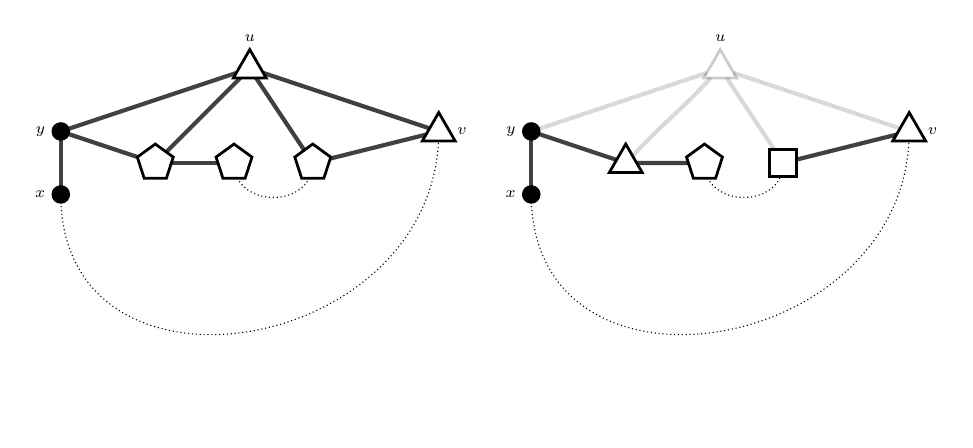
\begin{tikzpicture}
\begin{scope}[scale=0.8, every node/.append style={transform shape}]]
\draw[densely dotted] (3, 1) to [out=270,in=270,looseness=1.5] (-3, 0);
\draw[densely dotted] (-0.25, 0.5) to [out=270,in=270,looseness=1.5] (1.0, 0.5);

\VertexI[label=$x$, position=left, x=-3, y=0]{X}
\VertexI[label=$y$, position=left, x=-3, y=1]{Y}

\VertexIII[label=$u$, position=above, x=0, y=2]{U}
\VertexIII[label=$v$, position=right, x=3, y=1]{V}
\VertexV[x=-1.5, y=0.5]{u1}
\VertexV[x=-0.25, y=0.5]{u2}
\VertexV[x=1.0, y=0.5]{u3}

\Edge(X)(Y)
\Edge(Y)(U)
\Edge(U)(V)
\Edge(Y)(u1)
\Edge(u1)(u2)
\Edge(u3)(V)
\Edge(U)(u1)
\Edge(U)(u3)

\end{scope}

\begin{scope}[xshift=170, scale=0.8, every node/.append style={transform shape}]]
\draw[densely dotted] (3, 1) to [out=270,in=270,looseness=1.5] (-3, 0);
\draw[densely dotted] (-0.25, 0.5) to [out=270,in=270,looseness=1.5] (1.0, 0.5);

\VertexI[label=$x$, position=left, x=-3, y=0]{X}
\VertexI[label=$y$, position=left, x=-3, y=1]{Y}

\Vertex[label=$u$, position=above, x=0, y=2, color=white, style={regular polygon, regular polygon sides=3, opacity=0.2}]{U}
\VertexIII[label=$v$, position=right, x=3, y=1]{V}
\VertexIII[x=-1.5, y=0.5]{u1}
\VertexV[x=-0.25, y=0.5]{u2}
\VertexIV[x=1.0, y=0.5]{u3}

\Edge(X)(Y)
\Edge[opacity=0.2](Y)(U)
\Edge[opacity=0.2](U)(V)
\Edge(Y)(u1)
\Edge(u1)(u2)
\Edge(u3)(V)
\Edge[opacity=0.2](U)(u1)
\Edge[opacity=0.2](U)(u3)

\end{scope}
\end{tikzpicture}
\vspace{-1cm}
\caption{Illustration of Thomassen's reduction. At most $2$ colors are erased from the lists of $u$'s neighbors.}
\end{figure}

\end{proof}

\todo{Criticality definition. Discuss it}

In coloring problems, it is useful to consider when a precoloring of a subgraph
does not \emph{extend} to the entire graph, that is, there is no coloring
of the entire graph under certain constraints which agrees with the coloring 
of the subgraph. 




\begin{definition}[Extending]
	Let $G$ be a graph, $T \subseteq G$ a subgraph, and $L$ a list assignment
	for $G$. For an $L$-coloring $\phi$ of $T$, we say that $\phi$ \emph{extends}
	to an $L$-coloring of $G$ if there exists an $L$-coloring $\psi$ of $G$
s	such that $\phi(v) = \psi(v)$ for all $v \in V(T)$. 
	
\end{definition}

It is also interesting to consider graphs which are critical in this setting. To do so, we use the following definition (from \cite{fivelistcoloring2}):

\begin{definition}[$T$-critical]
	Let $G$, $T$, $L$ be as above. The graph $G$ is \emph{$T$-critical with respect to $L$} if for every proper subgraph $G' \subset G$ such that $T \subseteq G'$, there exists an $L$-coloring of $T$ that extends to an $L$-coloring of $G'$, but does not extend to an $L$-coloring of $G$. If the list assignment $L$ is clear from context, we just say \emph{$T$-critical}.
\end{definition}

\begin{definition}[$\phi$-critical]
	Let, $G$, $T$, $L$ be as above. The graph $G$ is $\phi$-critical for a coloring $\phi$ of $T$ if $\phi$ extends to every proper subgraph of $G$ containing $T$ but not to $G$.
\end{definition}

In a way similar to the general notion of criticality, we have that graphs for which colorings of $T$ do not extend contain a non-trivial $T$-critical subgraph:

\begin{lemma}
Let $G$ be a graph, $T$ a subgraph, and $L$ a list assignment for $G$. If there 
is an $L$-coloring $\phi$ of $T$ that does not extend to $G$, 
then $G$ contains a subgraph $H$ with $T \subsetneq H$ which 
is $\phi$-critical, and hence also $T$-critical with respect 
to $L\restriction_H$. 
\end{lemma}

\begin{proof}
Let $\phi$ be the coloring of $T$ that does not extend and let $H$ be a minimal subgraph 
of $G$ for which $\phi$ does not extend. Now note that $H$ is $\phi$-critical 
by construction.
\end{proof}

\begin{lemma}
\label{minimalsubgraphlemma}
Let $G$ be a graph, $T$ a subgraph, $L$ a list assignment for $G$, and $H \supseteq T$ 
a subgraph of $G$ which is minimal with respect to the following property: 
for every $L$-coloring $\phi$ of $T$ that extends to $H$, $\phi$ also extends to $G$. 
Then $H$ is $T$-critical.
\end{lemma}

\begin{proof}
Suppose not. Then, $H$ contains a proper subgraph $H'$ so that every $L$-coloring $\phi$ that extends to $H'$ also extends to $H$ and hence to $G$. But then $H'$ is a smaller subgraph with that property, contradiction. 
\end{proof}

We also have the following lemma from \cite{fivelistcoloring2}:

\begin{lemma}
\label{pregluinglemma}
Let $T$ be a subgraph of a graph $G$ such that $G$ is $T$-critical with respect to a list assignment $L$. Let $A, B \subseteq G$ be such that $A \cup B = G$ and $T \subseteq A$. Then $G[V(B)]$ is $A[V(A) \cap V(B)]$-critical.
\end{lemma}

\begin{proof} 
Let $G' = G[V(B)]$ and $S = A[V(A) \cap V(B)]$. If $G' = S$ there is nothing to say, suppose otherwise that $G' \neq S$ and note that therefore $G'$ contains an edge not in $S$ (in fact, all isolated vertices of $G'$ must be in $S$). Suppose for a contradiction that $G'$ is not $S$-critical. Then, by taking a maximal proper subgraph that defies the defintion, there exists an edge $e \in E(G') \setminus E(S)$ such that every $L$-coloring of $S$ that extends to $G' \setminus e$ also extends to $G'$. Since $G$ is $T$-critical and $e \not\in E(T)$, there exists a coloring $\phi\restriction_T$ of $T$ that extends to an $L$-coloring $\phi$ of $G \setminus e$, but does not extend to an $L$-coloring of $G$. However, by the choice of $e$, the restriction $\phi\restriction_S$ extends to an $L$-coloring $\phi'$ of $G'$. Let $\phi''$ be such that $\phi''(v) = \phi'(v) \, \forall v \in V(G')$ and $\phi''(v) = \phi(v) \, \forall v \in V(G) \setminus V(G')$. Now, since $A \cup B = G$, $\phi''$ is an $L$-coloring of $G$ extending $\phi\restriction_T$, a contradiction.
\end{proof}

For us, it will be more useful in this form: \todo{check if this is the best phrasing}

\begin{lemma}[Gluing Lemma]
\label{gluinglemma}
Let $T$ be a subgraph of a graph $G$ such that $G$ is $T$-critical with respect to a list assignment $L$. Let $A, B \subseteq G$ be such that $A \cup B = G$. Then $G[V(B)]$ is $(A[V(A) \cap V(B)] \cup T)$-critical.
\end{lemma}

\begin{proof} 
Apply \ref{pregluinglemma} to $A' = A \cup T$ and $B' = B$. 
\end{proof}

\missingfigure{Gluing lemma illustration}

The reason we decided to name it ``Gluing lemma'' in this work is that it is useful to visualize the graph $G$ as made of two separate pieces, $A$ and $B$, which are glued together along $A[V(A) \cap V(B)]$. In our approach we will frequently use the fact that all $T$-critical graphs can be ``decomposed'' in this way. 

\todo{Analogous results for List coloring}




\chapter{Critical Graphs on the Torus}

In this chapter we delve into the details of critical and list-critical graphs on the torus,
including Postle's approach for list-critical graphs on surfaces and Thomassen's approach
for $6$-critical graphs on the torus. 
From studying these, we develop our own, computer-aided approach
for $6$-list-critical graphs on the torus.

\section{An Overview of Postle's Approach}

Here we briefly explain Postle's approach in \cite{postlethesis} to obtain the result on the finiteness of 6-list-critical graphs in general surfaces, mentioning specially those intermediate results or definitions we will also use in our approach. The results obtained by Postle are very non-explicit in the sense that the (unspecified) constant in the size bounds for the graphs he obtains is extremely large and hence useless for our purpose of finding an explicit characterization. Nevertheless, given that our approach is primarily guided by this work we consider it of interest to provide a exposition of the main argument.

The results developed in \cite{postlethesis} in 2012 have been published successively in journal articles afterwards, often with improvements in exposition or in the strength of the result. We refer to the corresponding published article in the discussion of each particular result.

\subsection{Notation and Terminology}

Postle works mainly in a setting similar to the hypothesis of Thomassen's stronger theorem: list assignments $L$ which have list sizes of length at least $5$ for interior vertices and at least $3$ for exterior vertices with some exceptions. This setting is encapsulated in the concept of \emph{canvas}.

\begin{definition}[Canvas]
We say that $(G, S, L)$ is a \emph{canvas} if $G$ is a connected plane graph
 with outer walk $C$, $S$ is a subgraph of $C$, and $L$ is a list assignment
  such that $|L(v)| \geq 5 \, \forall v \in V(G) \setminus V(C)$ and
   $|L(v)| \geq 3 \, \forall v \in V(C) \setminus V(S)$. If $S$ is a path,
    we say $(G, S, L)$ is a \emph{path-canvas} or a \emph{wedge}. If $S = C$ and 
    $C$ is a cycle, then $(G, C, L)$ is a \emph{cycle-canvas}.
\end{definition} 



Note: in some places like \cite{fivelistcoloring2}, the term ``canvas'' is used for what Postle calls in \cite{postlethesis} ``cycle-canvas''.

We can restate Thomassen's Stronger Theorem in these terms:

\begin{theorem}
If $(G, P, L)$ is a path-canvas and $|V(P)| \leq 2$, then $G$ is $L$-colorable.
\end{theorem}

\begin{definition}[Critical canvas]
We say that a canvas $(G, S, L)$ is \emph{critical} if it is $S$-critical with respect to $L$.
\end{definition}

In the context of canvases, we usually talk of \emph{separating vertices} or \emph{separating
subgraphs} as graphs which, when removed, disconnect vertices of $S$ from other vertices in $S$.



\subsection{Variations on Thomassen's Condition}

Much of the technical work on Postle's thesis relies in a careful study of what happens if one varies the condition on \ref{thomassenstrongertheorem}. One of the most elegant (and also useful) results is the following strengthening to Thomassen's Stronger Theorem, originally conjectured by Hutchinson in \cite{hutchinson2012outerplanar}.

\begin{theorem}[Two Lists of Size Two Theorem \cite{fivelistcoloring1}]
\label{twolistsofsizetwo}
If $G$ is a plane graph with outer cycle $C$, $v_1, v_2 \in C$ and $L$ is a list assignment with $|L(v)| \geq 5$ for all $v \in V(G) \setminus V(C)$, $|L(v)| \geq 3$ for all $v \in V(C) \setminus \{v_1, v_2\}$, and $|L(v_1)| = |L(v_2)| = 2$, then $G$ is $L$-colorable. 
\end{theorem}

Or, in the language of canvases:

\begin{theorem}
If $(G, S, L)$ is a canvas with $|V(S)| = 2$ and $L(v) \geq 2$ for $v \in S$, then $G$ is $L$-colorable.
\end{theorem}

This theorem is not true when one of the two vertices has list of size $1$. In fact, Postle characterizes exactly when it fails:

\begin{definition}[Coloring Harmonica]
Let $G$ be a plane graph and $L$ a list assignment for $G$. Given an edge $uv$ and a vertex $w$ both from the outer face of $G$, we say that $(G, L)$ is a \emph{coloring harmonica from $uv$ to $w$} if either:

	\begin{itemize}
		\item $G$ is a triangle with vertex set $\{u, v, w\}$ and $L(u) = L(v) = L(w)$ with $|L(u)| = 2$, or
		\item There exists a vertex $z$ incident with the outer face of $G$ such that $uvz$ is a triangle in $G$, $L(u) = L(v) \subseteq L(z)$, $|L(u)| = |L(v)| = 2$, $|L(z)| = 3$, and the pair $(G', L')$ is a coloring harmonica from $z$ to $w$, where $G'$ is obtained by deleting \textbf{one or both} of the vertices $u$, $v$ and $L'$ is obtained from $L$ by $L'(z) = L(z) \setminus L(u)$ and $L'(x) = L(x)$ for all other vertices $z \neq x \in V(G')$.
	\end{itemize}

	Given two vertices $u, w$ in the outer face of $G$, we say $(G, L)$ is a \emph{coloring harmonica from $u$ to $w$} if there exist vertices $x, y$ incident with the outer face of $G$ such that $uxy$ is a triangle in $G$, $|L(u)| = 1$, $L(x) - L(u) = L(y) - L(u)$, $|L(x)-L(u)|=2$, and $(G', L')$ is a coloring harmonica from $xy$ to $w$, where $G'$ is obtained from $G$ by removing $u$, and $L'$ is obtained from $L$ by seting $L'(x) = L'(y) = L(x)-L(u)$ and $L'(z) = L(z)$ for every $z \in V(G') \setminus \{x, y\}$.


We say that $(G, L)$ is a coloring harmonica if it is a coloring harmonica from $uv$ to $w$ or a coloring harmonica from $u$ to $w$ for some $u, v, w$ as specified earlier.
\end{definition}

\missingfigure{harmonica}

See the example in (reference to figure) (from \cite{fivelistcoloring3}) for some clarity with respect to this mutually recursive definition. Note that the definition makes it clear that graphs which contain a coloring harmonica as a subgraph are not $L$-colorable. 

\begin{theorem}{One List of Size One and One List of Size Two Theorem \cite{fivelistcoloring3}}
Let $G$ be a plane graph with outer cycle $C$, let $p_1, p_2 \in V(C)$, and let
$L$ be a list assignment with $|L(v)| \geq 5$ for all $v \in V(G) \setminus V(C)$, $|L(v)| \geq 3$ for all
$v \in V (C) \setminus \{p_1 , p_2\}$, $|L(p_1)| \geq 1$ and $|L(p_2)| \geq 2$. Then $G$ is $L$-colorable if and only if the pair $(G, L)$ does not contain a coloring harmonica from $p_1$ to $p_2$.
\end{theorem}

Studying conditions of the sizes of the lists in the boundary in which the graph is not $L$-colorable like this one is also useful, because such conditions arise when dealing when reductions and therefore characterizing which are the critical graphs in such settings can give fruitful results.

Thomassen already studied when does the coloring of a path of length $2$ not extend:

\begin{definition}[Bellows]
	We say that a path-canvas $(G, P, L)$ with $P = p_0p_1p_2$ is a \emph{bellows} (terminology from \cite{postlethesis}) or a \emph{generalized wheel} (terminology from \cite{thomassenexponentiallymany5listcolorings}) if either:
	\begin{itemize}
		\item $G$ has no interior vertices and its edge set consists of the edges of the outer cycle plus all edges from $p_1$ to vertices of the outer cycle. In this case, we say that $(G, P, L)$ is a \emph{fan}.
		\item $G$ has one interior vertex $u$ and its edge set consists of the edges of the outer cycle plus all edges from $u$ to vertices of the outer cycle. In this case, we say that $(G, P, L)$ is a \emph{turbofan}.
		\item $G$ can be formed by gluing two smaller bellows from the edges $p_1p_2$ and $p_0p_1$ respectively. 
	\end{itemize}
\end{definition}

\missingfigure{bellows}


\begin{theorem}[\cite{thomassenexponentiallymany5listcolorings}, Theorem 3]
	If $T = (G, P, L)$ is a path-canvas with path length $2$, then $G$ is $L$-colorable unless $T$ has a bellows as a subcanvas.
\end{theorem}

Postle studies when the coloring of two paths of length $1$ does not extend. He finds the following obstruction:

\begin{definition}[Accordion]
	We say that a canvas $T = (G, P_1 \cup P_2, L)$ with $P_1, P_2$ distinct paths of length $1$ is an \emph{accordion} with \emph{ends} $P_1, P_2$ if $T$ is a bellows with $P_1 \cup P_2$ path of length $2$ or $T$ is the gluing of two smaller accordions $T_1 = (G_1, P_1 \cup U, L)$ with ends $P_1, U$ and $T_2 = (G_2, P_2 \cup U, L)$ with ends $U$, $P_2$ along a chord $U = u_1u_2$ where $|L(u_1)|, |L(u_2)| \leq 3$.
\end{definition}

The main result he obtains is that if the two paths are sufficiently far apart, then the graph contains a proportionally large accordion or a coloring harmonica as a subgraph.

\begin{theorem}[Bottleneck Theorem, loosely stated]
\label{bottlenecktheorem}
If $T = (G, P \cup P_0 , L)$ is a canvas with $P, P_0$ distinct edges of $C$ with $d(P, P_0) \geq 14$, then either there exists an $L$-coloring of $G$, or there exists a subcanvas $(G_0 , U_1 \cup U_2 , L)$ of $T$ where $d_{G_0} (U_1, U_2) = \Omega(d_G (P, P_0))$ which is an accordion or a coloring harmonica.
\end{theorem}

This result, along with coloring and structural properties of accordions and harmonicas, is often used as a technical lemma when proving the following results.

\subsection{Linear Bound on Critical Cycle-Canvases}

Postle proves the following result:

\begin{theorem}[\cite{fivelistcoloring2}]
\label{linearboundcycletheorem}
Let $G$ be a plane graph with outer cycle $C$ and $L$ a $5$-lis-assignment for $G$. Let $H$ be a minimal subgraph of $G$ such that every $L$-coloring of $C$ that extends to an $L$-coloring of $H$ also extends to an $L$-coloring of $G$. Then $H$ has at most $19|V(C)|$ vertices.
\end{theorem}

Or, equivalently stated in the language of critical canvases:

\begin{theorem}
If $(G, C, L)$ is a critical cycle-canvas, then $|V(G)| \leq 19 |V(C)|$.
\end{theorem}

The equivalence of the two statements is given by \ref{minimalsubgraphlemma}. This result is interesting in its own right because by \ref{gluinglemma}, all faces of a $T$-critical graph which do not separate vertices from $T$ are in fact critical cycle-canvases, and therefore what the result tells us is that for such graphs there is only finitely many kinds of faces that can appear for each given cycle length. This gives us a lot of information of how critical graphs look like. 

A first observation that can be made is that critical cycle-canvases (in which $C$ is indeed a simple cycle) are $2$-connected, so each face is bounded by a cycle:

\begin{lemma}
If $(G, C, L)$ is a critical cycle-canvas, then it is $2$-connected.
\end{lemma}

\begin{proof}
If $G$ is not $2$-connected, then there exist subgraphs $A, B$ such that $A \cup B = G$ with $|V(A) \cap V(B)| \leq 1$ and $|V(B) \setminus V(A)| \geq 1$. Assume $C \subseteq A$ and apply \ref{gluinglemma} to get that $B$ is $A[V(A) \cap V(B)]$-critical, contradicting \ref{thomassenstrongertheorem}.
\end{proof}

The key result in Postle's proof of the linear bound for cycles is the following theorem about the structure of critical cycle-canvases:

\begin{theorem}[Cycle Chord or Tripod Theorem]
\label{cyclechordtripodtheorem}
If $(G, C, L)$ is a critical cycle-canvas, then either

\begin{enumerate}
\item $C$ has a chord in $G$, or
\item there exists a vertex $v \in V(G) \ V(C)$ with at least three neighbors on $C$ such that at most one of the faces of $G[\{v\} \cup V(C)]$ includes a vertex or edge of $G$. 
\end{enumerate}
\end{theorem}

Using this result, Postle carefully examines what happens near the boundary cycle in order to define some quantities related to sums of lengths of faces and proves that certain inequalities with those quantites are mantained when adding tripods in critical canvases. 



\subsection{The Two Precolored Triangles Theorem}

Next, Postle proves the following theorem:

\begin{theorem}
	There exists $d$ such that the following holds.
	Let $G$ be a planar graph and $T_1, T_2$ triangles in $G$ at distance at least $d$. Let $L$ be a $5$-list-assignment of $G$. Then, every $L$-coloring of $T_1 \cup T_2$ extends to an $L$-coloring of $G$.
\end{theorem}

(Postle refers to the graphs with two precolored triangles and all other vertices with list sizes
at least $5$ as \emph{prism-canvases}, even though they are not a type of canvas).

The value of $d$ that Postle obtains is not explicitly stated, but it is on the order of $100$. However, we conjecture that $4$ or $5$ suffices.

\begin{conjecture}
\label{twotriangleconjecture}
Let $G$ be a planar graph and $T_1, T_2$ triangles in $G$ at distance at least $5$. Let $L$ be a $5$-list-assignment of $G$. Then, every $L$-coloring of $T_1 \cup T_2$ extends to an $L$-coloring of $G$.
\end{conjecture}

The argument that Postle uses to prove his result is as follows. First, he proves that one can precolor a path between the two triangles in such a way that, when deleting the path and deleting the corresponding colors from the lists of neighboring vertices, all remaining non-precolored vertices have lists of size at least $3$. The proof of this begins with the simple observation that each vertex outside a shortest path has at most $3$ neighbors inside the path. Using planarity properties, a shortest path can be found so that it can be colored in such a way that the vertices with $3$ neighbors inside the path only see two different colors from their lists.

After precoloring and deleting the path between the two triangles, a canvas $(G, P_1 \cup P_2, L)$ is obtained. If there was a precoloring of the triangles that did not extend, then the canvas contains a critical canvas, and by \ref{bottlenecktheorem} it contains a proportionally long accordion or harmonica. Postle proves that this (together with some technical details related to how the path between the triangles was chosen) implies that in the original graph there must be a long chain of separating triangles so that the graph between each separating triangle pertains to one of three very specific types, which he calls tetrahedral, octahedral or hexadecahedral bands. 

\todo{check if I defined separating triangle in introduction}

Finally, he proves that for a sufficiently long chain of this type, any precoloring of the innermost and outermost triangles extends to the whole chain. This proves the theorem, because of the following observation:

\begin{proposition}
	Let $G$ be a plane graph with $L$ a list assignment, $T_1$, $T_2$ 
	two facial triangles with $T_1$ bounding the infinite face of $G$, 
	and $T'_1$, $T'_2$ two triangles such that $T'_1$ is a separating 
	triangle between $T_1$ and $T'_2$ and $T'_2$ is a separating 
	triangle between $T'_1$ and $T_2$. Denote by $G[T'_1, T'_2]$ the 
	subgraph comprised between the two triangles $T'_1, T'_2$.  
	If there exists some $L$-coloring of $T_1 \cup T_2$ that does not 
	extend to $G$, then there exists some $L$-coloring of $T'_1 \cup T'_2$ 
	that does not extend to $G[T'_1, T'_2]$.
\end{proposition}

\begin{proof}
	By \ref{thomassenstrongertheorem}, the coloring on $T_1$ extends to 
	$G[T_1, T'_1]$ and the coloring on $T_2$ extends to $G[T'_2, T_2]$. 
	The coloring of $T'_1 \cup T'_2$ given by this extensions can not 
	extend to $G[T'_1, T'_2]$ by the assumption that the original coloring 
	of $T_1 \cup T_2$ did not extend to $G$.
\end{proof}

\subsection{Cylinder-Canvases and Hyperbolic Families}

Finally, Postle generalizes the previous setting of critical prism-canvases to \emph{critical cylinder-
canvases}, where a cylinder-canvas is like a prism-canvas but the precolored cycles can have length
greater than $3$. It generalizes Theorem \ref{twoprecoloredtrianglestheorem} by showing that for
every pair of cycle lengths, there exists a distance $d$ (depending logarithmically on the cycle sizes)
so that all critical cylinder-canvases have the cycles at distance at most $d$. It also generalizes
Theorem \ref{linearboundcycletheorem} by showing that critical cylinder-canvases have a bound
on their size linear in the sum of the cycle lengths.

Then, he defines \emph{hyperbolic families}: families of graphs embedded in surfaces which have
certain properties related to having planar graphs resulting from performing \emph{excisions} in
the surface always having bounded size. We do not delve into the details because the topological
arguments for the general case are not of interest for us, but we will explain some similar
operations on the torus in the section explaining our approach. 

The idea here is that the linear bounds on the cycle-canvases and the cylinder-canvases make the 
$6$-list-critical graphs on the torus be an hyperbolic family. Then, the result we want about
the finiteness of $6$-list-critical graphs is proven for the more general setting of hyperbolic
families. In fact, it is proven that the number of vertices of such is bounded linearly by the genus 
of the surface.

The general setting of hyperbolic surfaces allows Postle to prove more properties and bounds of
$6$-list-critical graphs on the torus, such as:

\begin{theorem}
\label{edgewidththeorem}
Let $G$ be a graph 2-cell-embedded in a surface $\Sigma$ and let $L$ be a $5$-list-assignment.
If $ew(G) \geq O(\log g(\Sigma))$, then $G$ is $L$-colorable. 

\end{theorem}





\section{Critical Graphs on the Torus for (usual) Vertex Coloring}

In this section we discuss the result from Thomassen in \cite{thomassentorus} that characterizes the critical graphs for $5$-coloring (not $5$-list-coloring) on the torus.

\subsection{The Critical Graphs}

\begin{theorem}[\cite{thomassentorus}]
	\label{thomassentorustheorem}
	A graph $G$ embeddable on the torus is $5$-colorable if and only if 
	it does not contain the following subgraphs:
	\begin{itemize}
		\item $K_6$.
		\item $C_3 + C_5$.
		\item $K_2 + H_7$, where $H_7$ is a $7$-vertex graph known as the \emph{Moser spindle}.
		\item $T_{11}$, where $T_{11}$ is a triangulation of the torus with $11$ vertices.
	\end{itemize}
	Where $+$ denotes the join of two graphs: their disjoint union with 
	all pairs of vertices from different graphs joined by edges.
\end{theorem} 


\begin{figure}
\centering
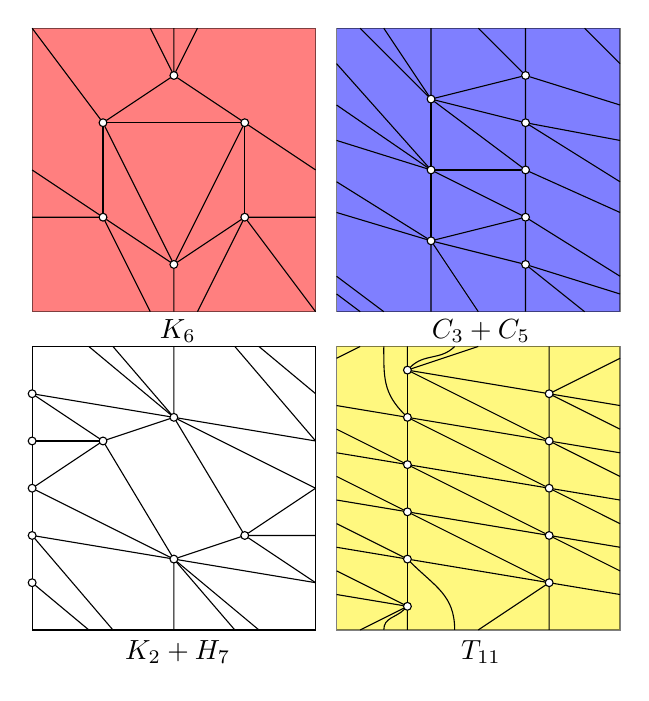
\begin{tikzpicture}[main/.style = {draw, circle, fill=white}]

\begin{scope}[scale=0.3, every node/.append style={transform shape}]]
\draw[draw=black, fill=red, opacity=0.5] (0, 0) rectangle (12, 12);




\node[main] (A1) at (6, 10) {};
\node[main] (A2) at (3, 4) {};
\node[main] (A3) at (9, 4) {};

\node[main] (B1) at (6, 2){};
\node[main] (B2) at (9, 8) {};
\node[main] (B3) at (3, 8) {};


\draw (A1) -- (B2);
\draw (B2) -- (A3);
\draw (A3) -- (B1);
\draw (B1) -- (A2);
\draw (A2) -- (B3);
\draw (B3) -- (A1);

\draw (A1) -- (6, 12);
\draw (6, 0) -- (B1);
%\draw (A2) -- (0, 0);
%\draw (12, 12) -- (B2);
\draw (A3) -- (12, 0);
\draw (0, 12) -- (B3);

\draw (A2) -- (0, 6);
\draw (12, 6) -- (B2);

\draw (B1) -- (B2);
\draw (B2) -- (B3);
\draw (B3) -- (B1);

\draw (A2) -- (0, 4);
\draw (12, 4) -- (A3);
\draw (A2) -- (5, 0);
\draw (5, 12) -- (A1);
\draw (A3) -- (7, 0);
\draw (7, 12) -- (A1);


\end{scope}

\begin{scope}[xshift=110, scale=0.3, every node/.append style={transform shape}]]
\draw[draw=black, fill=blue, opacity=0.5] (0, 0) rectangle (12, 12);




\node[main] (A1) at (4, 9) {};
\node[main] (A2) at (4, 6) {};
\node[main] (A3) at (4, 3) {};



\node[main] (B1) at (8, 10){};
\node[main] (B2) at (8, 8) {};
\node[main] (B3) at (8, 6) {};
\node[main] (B4) at (8, 4) {};
\node[main] (B5) at (8, 2) {};


\draw (4, 12) -- (A1);
\draw (A1) -- (A2);
\draw (A2) -- (A3);
\draw (A3) -- (4, 0);

\draw (8, 12) -- (B1);
\draw (B1) -- (B2);
\draw (B2) -- (B3);
\draw (B3) -- (B4);
\draw (B4) -- (B5);
\draw (B5) -- (8, 0);

\draw (A1) -- (B1);
\draw (A1) -- (B2);
\draw (A1) -- (B3);
\draw (A1) -- (2, 12);
\draw (2, 0) -- (0, 1.5);
\draw (12, 1.5) -- (B4);
\draw (A1) -- (1, 12);
\draw (1, 0) -- (0, 0.75);
\draw (12, 0.75) -- (B5);

\draw (A2) -- (B3);
\draw (A2) -- (B4);
\draw (A2) -- (0, 10.5);
\draw (12, 10.5) -- (10.5, 12);
\draw (10.5, 0) -- (B5);
\draw (A2) -- (0, 8.75);
\draw (12, 8.75) -- (B1);
\draw (A2) -- (0, 7.25);
\draw (12, 7.25) -- (B2);


\draw (A3) -- (B4);
\draw (A3) -- (B5);
\draw (A3) -- (6, 0);
\draw (6, 12) -- (B1);
\draw (A3) -- (0, 5.5);
\draw (12, 5.5) -- (B2);
\draw (A3) -- (0, 4.2);
\draw (12, 4.2) -- (B3);
\end{scope}


\begin{scope}[yshift=-115, scale=0.3, every node/.append style={transform shape}]]
\draw[draw=black] (0, 0) rectangle (12, 12);




\node[main] (A1) at (0, 8) {};
\node[main] (A2) at (0, 10) {};
\node[main] (A3) at (0, 2) {};
\node[main] (A4) at (0, 4) {};
\node[main] (A5) at (0, 6) {};

\coordinate[] (A1c) at (12, 8) {};
\coordinate[] (A2c) at (12, 10) {};
\coordinate[] (A3c) at (12, 2) {};
\coordinate[] (A4c) at (12, 4) {};
\coordinate[] (A5c) at (12, 6) {};

\node[main] (H1) at (3, 8) {};
\node[main] (H2) at (9, 4) {};

\node[main] (K1) at (6, 9) {};
\node[main] (K2) at (6, 3) {};




\draw (A1) -- (A2);
\draw (A2) -- (0, 12);
\draw (0, 0) -- (A3);
\draw (A3) -- (A4);
\draw (A4) -- (A5);
\draw (A5) -- (A1);

\draw (H1) -- (A1);
\draw (H1) -- (A2);
\draw (H1) -- (A5);

\draw (H2) -- (A3c);
\draw (H2) -- (A4c);
\draw (H2) -- (A5c);

\draw (K1) -- (A2);
\draw (K1) -- (A1c);
\draw (K1) -- (A5c);
\draw (K1) -- (H1);
\draw (K1) -- (H2);
\draw (K1) -- (3.42, 12);
\draw (3.42, 0) -- (A4);
\draw (K1) -- (2.4, 12);
\draw (2.4, 0) -- (A3);

\draw (K2) -- (A5);
\draw (K2) -- (A4);
\draw (K2) -- (A3c);
\draw (K2) -- (H1);
\draw (K2) -- (H2);
\draw (K2) -- (12-3.42, 0);
\draw (12-3.42, 12) -- (A1c);
\draw (K2) -- (12-2.4, 0);
\draw (12-2.4, 12) -- (A2c);


\draw (K1) -- (6, 12);
\draw (6, 0) -- (K2);

\end{scope}

\begin{scope}[xshift=110, yshift=-115, scale=0.3, every node/.append style={transform shape}]]
\draw[draw=black, fill=yellow, opacity=0.5] (0, 0) rectangle (12, 12);




\node[main] (A0) at (3, 11) {};
\node[main] (A1) at (3, 9) {};
\node[main] (A2) at (3, 7) {};
\node[main] (A3) at (3, 5) {};
\node[main] (A4) at (3, 3) {};
\node[main] (A5) at (3, 1) {};

\node[main] (B0) at (9, 10) {};
\node[main] (B1) at (9, 8) {};
\node[main] (B2) at (9, 6) {};
\node[main] (B3) at (9, 4) {};
\node[main] (B4) at (9, 2) {};

\draw (A0) -- (A1);
\draw (A1) -- (A2);
\draw (A2) -- (A3);
\draw (A3) -- (A4);
\draw (A4) -- (A5);

\draw (B0) -- (B1);
\draw (B1) -- (B2);
\draw (B2) -- (B3);
\draw (B3) -- (B4);

\draw (A0) -- (B0);
\draw (A0) -- (B1);
\draw (A1) -- (B1);
\draw (A1) -- (B2);
\draw (A2) -- (B2);
\draw (A2) -- (B3);
\draw (A3) -- (B3);
\draw (A3) -- (B4);
\draw (A4) -- (B4);

\draw (B0) -- (12, 9.5);
\draw (0, 9.5) -- (A1);
\draw (B0) -- (12, 8.5);
\draw (0, 8.5) -- (A2);
\draw (B1) -- (12, 7.5);
\draw (0, 7.5) -- (A2);
\draw (B1) -- (12, 6.5);
\draw (0, 6.5) -- (A3);
\draw (B2) -- (12, 5.5);
\draw (0, 5.5) -- (A3);
\draw (B2) -- (12, 4.5);
\draw (0, 4.5) -- (A4);
\draw (B3) -- (12, 3.5);
\draw (0, 3.5) -- (A4);
\draw (B3) -- (12, 2.5);
\draw (0, 2.5) -- (A5);
\draw (B4) -- (12, 1.5);
\draw (0, 1.5) -- (A5);

\draw (A4) to [out=-45, in=90, looseness=1.1] (5, 0);

\draw (5, 12) to [out = -135, in = 45, looseness=1.05] (A0);

\draw (B4) -- (6, 0);
\draw (6, 12) -- (A0);
\draw (B4) -- (9, 0);
\draw (9, 12) -- (B0);

\draw (A5) -- (3, 0);
\draw (3, 12) -- (A0);
\draw (A5) to [out=-135, in = 90, looseness=1.1] (2, 0);
\draw (2, 12) to [out=-90, in =135, looseness=1.1] (A1);
\draw (A5) -- (1, 0);
\draw (1, 12) -- (0, 11.5);
\draw (12, 11.5) -- (B0);

\end{scope}

\node[] at (1.85, -0.25) {$K_6$};
\node[] at (5.70, -0.25) {$C_3+C_5$};
\node[] at (1.85, -4.32) {$K_2+H_7$};
\node[] at (5.70, -4.32) {$T_{11}$};
\end{tikzpicture}
\caption{$6$-critical graphs embedded on the torus.}
\end{figure}

If a graph is not $5$-colorable, it is not $5$-list-colorable, so all graphs 
that contain any of the above subgraphs are not $5$-list-colorable. 
We conjecture that this characterizes the $5$-list-colorable graphs on the torus too:

\begin{conjecture}
\label{torusconjecture}
A graph $G$ embeddable on the torus is $5$-list-colorable if and only if 
it does not contain the following subgraphs: $K_6$, $C_3 + C_5$, $K_2 + H_7$, $T_{11}$.
\end{conjecture}

This means that those are the minimal $6$-list-critical graphs on the torus. Note 
that there may be additional $6$-list-critical graphs embeddable on the torus, but what we are conjecturing is that they all 
contain those subgraphs. For example:

\begin{observation}
$K_7$ is $6$-list-critical.
\end{observation}

\begin{proof}
Consider the following $5$-list-assignment for $K_7$: $L(v_1) = L(v_2) = L(v_3) = L(v_4) = L(v_5) = \{1, 2, 3, 4, 5\}$, 
$L(v_6) = L(v_7) = \{1, 2, 3, 4, 6\}$. $K_7$ is not $L$-colorable, since there are only $6$ available colors. 
But any subgraph is $L$-colorable. Let's give a coloring $\phi$ for $K_7 \setminus v_iv_j$. If $i, j \leq 5$, 
then setting $\phi(v_i) = \phi(v_j) = 5$ and $\phi(v_7) = 6$ leaves $4$ vertices to be colored with $4$ colors. 
If $i \leq 5$ and $j \geq 6$, then setting $\phi(v_i) = \phi(v_j) = 1$, $\phi(v_{13-j}) = 6$ leaves $4$ vertices 
to be colored with $4$ colors. If $\{i, j\} = \{6, 7\}$, then $\phi(v_i) = \phi(v_j) = 6$ leaves $5$ vertices 
to be colored with $5$ colors.

Hence, $K_7$ is $L$-critical for a $5$-list-assignment $L$, and is therefore $6$-list-critical.
\end{proof}

\subsection{An Overview of Thomassen's Approach}

Thomassen's article where he characterizes the graphs on the torus (\cite{thomassentorus}) predates 
his result on finitely many $6$-critical graphs for all surfaces (\cite{thomassenfixedsurface}). 
For the characterization of $6$-critical graphs on the torus, he only uses elementary, relatively 
straighforward arguments that work on specifically in the torus. We briefly summarize his 
approach here in order to discuss which arguments can be reused for the list-coloring case. 

First, Thomassen considers the case when the minimum degree is at least $6$. 

\begin{proposition}
If a graph $G$ embedded on the torus has $\delta(G) \geq 6$, then:

\begin{enumerate}
	\item $G$ is $6$-regular.
	\item $G$ is a triangulation of the torus.
\end{enumerate}
\end{proposition}

\begin{proof}
We apply Euler's formula: let $V, E, F$ be the number of vertices, edges and faces in the embedding, respectively. 
We have that $\delta(G) \geq 6 \implies V \leq \frac{1}{3} E$ with equality iff $G$ is $6$-regular, and $F \leq \frac{2}{3}E$ 
with equality iff $G$ is a triangulation. Then $0 = V - E + F \leq \frac{1}{3}E - E + \frac{2}{3}E = 0$, so we have equality on both inequalities.
\end{proof}

Using the proposition above, Thomassen then proves the following:

\begin{proposition}[3.2 in \cite{thomassentorus}]
Let $G$ be a $6$-regular graph on the torus. If $G$ contains a vertex $v$, such that $\{v\} \cup N(v)$ induces a nonplanar graph, then $G = K_7$ or $G$ is obtained from $K_8$ or $K_9$ by deleting the edges of a $1$-regular or $2$-regular subgraph.
\end{proposition}

The study of $6$-regular graphs on the torus without vertices whose neighborhood induces a nonplanar graph was already done by Thomassen in his previous paper \cite{thomassentilings}, in the context of finding all tilings of the torus in order to prove a conjecture by Babai about vertex-transitive graphs. 

He obtains the following result:

\begin{theorem}
Let $G$ be a graph embedded on the torus with $\delta(G) \geq 6$. Then $G$ is $5$-colorable 
unless $G = K_7$ or $G = T_{11}$.
\end{theorem}

This part of the argument is the one that can be generalized to list coloring, but it is not
useful to our approach, so we don't delve into the details. 

Let us now describe Thomassen's argument for 
general graphs.

He assumes a minimum counterexample $G_0$ to \ref{thomassentorustheorem} (the counterexample has
minimum number of vertices, maximum number of edges restricted to that, and some other assumptions 
about details we will not discuss here). By the previous result, 
there must be a vertex $v_0 \in V(G_0)$ with degree $\leq 5$, and the degree of $v_0$ is in 
fact equal to $5$ by minimality of the counterexample. 

Consider two vertices $x, y \in N(v_0)$ which are not adjacent (if all the vertices of 
$N(v_0)$ were adjacent, then $G_0$ would contain $K_6$, a contradiction). Let $G_{xy}$ be 
the graph obtained from $G_0 \setminus v_0$ by identifying the vertices $x$ and $y$. 
$G_{xy}$ can be embedded in the torus by modifying the embedding of $G_0$. If $G_{xy}$ 
were $5$-colorable, then we would have a $5$-coloring of $G_0$ by assigning the same color 
to $x$ and $y$ and coloring $v_0$ with a color not appearing in its $5$ neighbors. 
Hence, $G_{xy}$ is not $5$-colorable and by minimality of our counterexample it 
contains $K_6$, $C_3 + C_5$, $K_2 + H_7$ or $T_{11}$.

The above argument works for all pairs $x, y$ of non-adjacent vertices in $N(v_0)$, so potentially 
we can have many different obstructions for each of the corresponding $G_{xy}$ subgraphs. 
But we can prove that, by minimality, there can not be much else in $G_0$ apart from these
obstructions arising from all the $G_{xy}$ subgraphs. More precisely:  

\begin{proposition}
	\label{g0proposition}
	For any non-adjacent $x, y \in N(v_0)$, let $G'_{xy}$ a copy of 
	$K_6$, $C_3 + C_5$, $K_2 + H_7$ or $T_{11}$ in $G_{xy}$, and let $G''_{xy}$ be the induced
	subgraph of $G_{xy}$ by the vertex set of $G'_{xy}$. Then $G_0$ consists of $v_0$, $N(v_0)$, 
	the edges between vertices of $\{v_0\} \cup N(v_0)$, and the union over all non-adjacent 
	$x, y \in N(v_0)$ of the graph obtained from $G''_{xy}$ by splitting the contracted vertex
	into $x$ and $y$.  
\end{proposition}

\begin{proof}
We will prove that the graph described above, which is a subgraph of $G_0$, is not $5$-colorable. 
This means, by the assumptions of minimality of vertices and maximality of edges, that $G_0$ is
in fact equal to that subgraph. 

If the subgraph had a $5$-coloring, then two non-adjacent vertices $x, y$ of $N(v_0)$ would 
have the same color. But by then identifying the two vertices we can get a $5$-coloring 
of $G''_{xy}$, which contains the non-$5$-colorable subgraph $G'_{xy}$, contradiction.

\end{proof}

Note that, since the maximum number of vertices in a critical graph is $11$, this means that
$G_0$ has at most $(11 - 1) \cdot \binom{5}{2} + 6 = 106$ vertices, and hence what remains
is a finite problem.

Thomassen uses some more arguments to narrow down the remaining possibilities for $G_0$, but
we can already see an important point of failure of this argument for list-coloring: in the 
proof of \ref{g0proposition}, it is used that a necessary and sufficient condition for a coloring
of $G_0 \setminus v_0$ to extend to $v_0$ is that two neighbors of $v_0$ have the same color.
In list coloring, this condition is not necessary. So we cannot conclude that the minimum 
counterexample is the union of the graphs induced by the obstructions in $G_{xy}$ and the 
argument breaks down here. 











\section{Our Approach}

The bounds on the size of $6$-list-critical graphs on the torus given by Postle's approach are 
way too large to be of any use to us in our search of the explicit list for the torus. However, 
we can take inspiration in his approach and in particular in how it was useful to carefully study
critical canvases. The key modification is that, instead of proving abstract bounds for sizes
of critical canvases as in Theorem \ref{linearboundcycletheorem}, we will be working with the 
explicit, full list of critical canvases of a certain type and size. 

In order to obtain those canvases, we will be using computer search, so this will be a 
computer-aided proof, like the Four Color Theorem's (but using very different techniques). The 
reason we consider it feasible to perform this search is that results like 
Theorem \ref{cyclechordortripodtheorem} give very structured descriptions of 
critical canvases - so we don't face enormously huge space of searching among
all the planar graphs with a given size bound, but instead have a much more restricted
search space. 

Once we have generated some critical canvases, our idea is to take advantage of them in a way 
similar to Postle's approach - but this time, 
since we will work with the explicit canvases instead of loose bounds, the hope is that we
can use them to obtain also the explicit list of $6$-list-critical graphs. 

Since the torus is not a complicated surface, there are simple manipulations 
that relate $6$-list-critical graphs on the torus with critical prism-canvases
 and cycle-canvases, as we will see now. 

\subsection{Cutting Through a Non-Contractible Cycle}

Consider the torus $S_1$. If one cuts through non-contractible curve
\todo{check if this is the appropiate term} 
one obtains a cylinder,
which can then be projected to the plane. 

We can do this to get planar graphs from graphs $2$-cell-embedded on the torus: we can cut 
through a non-contractible cycle, duplicate the vertices on the cycle so they appear on both
sides of the resulting cylinder, and then project this cylinder into the plane. See Figure \ref{fig:k6criticalprismcanvas} for an example with $K_6$, one of the $6$-critical graphs
embedded on the torus. 

\begin{figure}
\label{fig:k6criticalprismcanvas}
\centering
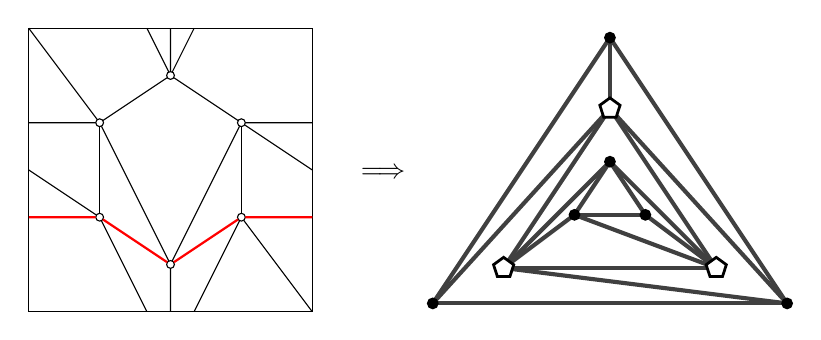
\begin{tikzpicture}[main/.style = {draw, circle, fill=white}]

\begin{scope}[scale=0.3, every node/.append style={transform shape}]]
\draw[draw=black] (0, 0) rectangle (12, 12);

\node[main] (A1) at (6, 10) {};
\node[main] (A2) at (3, 4) {};
\node[main] (A3) at (9, 4) {};

\node[main] (B1) at (6, 2){};
\node[main] (B2) at (9, 8) {};
\node[main] (B3) at (3, 8) {};


\draw (A1) -- (B2);
\draw (B2) -- (A3);
\draw [red,thick] (A3) -- (B1);
\draw [red,thick] (B1) -- (A2);
\draw (A2) -- (B3);
\draw (B3) -- (A1);

\draw (A1) -- (6, 12);
\draw (6, 0) -- (B1);
%\draw (A2) -- (0, 0);
%\draw (12, 12) -- (B2);
\draw (A3) -- (12, 0);
\draw (0, 12) -- (B3);

\draw (A2) -- (0, 6);
\draw (12, 6) -- (B2);

\draw (B1) -- (B2);
%\draw (B2) -- (B3);
\draw (B2) -- (12, 8);
\draw (0, 8) -- (B3);
\draw (B3) -- (B1);

\draw [red,thick] (A2) -- (0, 4);
\draw [red,thick](12, 4) -- (A3);
\draw (A2) -- (5, 0);
\draw (5, 12) -- (A1);
\draw (A3) -- (7, 0);
\draw (7, 12) -- (A1);


\end{scope}

\node () at (4.5, 1.75) {$\implies$};

\begin{scope}[xshift=210,yshift=35, scale=0.45, every node/.append style={transform shape}]
\VertexI[x=-5, y=-2.5] {A1}
\VertexI[x=5,  y=-2.5] {A2}
\VertexI[x=0,  y=5] {A3}

\VertexV[x=-3, y=-1.5] {B1}
\VertexV[x=3,  y=-1.5] {B2}
\VertexV[x=0,  y=3] {B3}

\VertexI[x=-1, y=0] {C1}
\VertexI[x=1,  y=0] {C2}
\VertexI[x=0,  y=1.5] {C3}

\Edge(A1)(A2)
\Edge(A2)(A3)
\Edge(A3)(A1)

\Edge(C1)(C2)
\Edge(C2)(C3)
\Edge(C3)(C1)

\Edge(A1)(B3)
\Edge(A2)(B3)
\Edge(A3)(B3)
\Edge(A2)(B1)

\Edge(B1)(B3)
\Edge(B2)(B3)
\Edge(B1)(B2)

\Edge(B1)(C3)
\Edge(B1)(C1)
\Edge(B2)(C1)
\Edge(B2)(C2)
\Edge(B2)(C3)


\end{scope}
\end{tikzpicture}
\caption{Cutting $K_6$ into a critical prism-canvas.}
\end{figure}

The reason why this is useful to us is the following observation:

\begin{observation}
Let $G$ be a graph embedded on the torus, let $G'$ be a graph obtained by 
this procedure from $G$, let $C_1, C_2$ be the two cycles of $G;$ corresponding to the
non-contractible cycle $C$ of $G$ we cut through, let $L$ be a list assignment for $G$ and let
$L'$ be the corresponding list assignment for $G'$ (with the same lists for all vertices,
duplicated for $C_1$ and $C_2$).

If $G$ is $L$-critical, then $G'$ is $(C_1 \cup C_2)$-critical with respect to the
list assignment $L'$.
\end{observation}

\begin{proof}
Consider a subgraph $(C_1 \cup C_2) \subseteq H' \subset G'$ and
the corresponding subgraph $C \subseteq H \subset G$. 
By $L$-criticality of $G$, $H$ is $L$-colorable with a coloring $\phi$.
Consider the corresponding coloring $\phi'$ of $H'$.
 Then, $\phi'_{\restriction_{C_1 \cup C_2}}$
is a coloring of $(C_1 \cup C_2)$ which extends to $H'$ but not to $G'$, since if it extended
to $G'$ we would have a $L'$-coloring of $G'$ in which the corresponding vertices of $C_1$ and
$C_2$ have the same colors and therefore we would be able to retrieve an $L$-coloring of $G$.
\end{proof}

This, together with Theorem \ref{twotriangletheorem}, already places a restriction on how the
$6$-list-critical graphs on the torus can be: if the graph has a non-contractible triangle, then
it must also have a not too large non-contractible cycle not homotopically equivalent to 
the non-contractible triangle, since if the two precolored triangles are at distance $d$ in the
resulting planar graph, then there is such a non-contractible cycle of length $\leq d+1$ in the
original graph. 

An interesting implication is also that we can do the process backwards: if we have a critical 
prism-canvas, we can ``fuse the two triangles'' to get a graph on the torus which is 
\emph{possibly} $6$-list-critical.   

\subsection{Cutting Across Two Non-Contractible Cycles}

Instead of just cutting through one non-contractible cycle to get a cylinder and project it to the
plane, we can cut through two non-homotopically-equivalent non-contractible cycles to get the 
plane, as in Figure \ref{fig:twocycles_illustration}. This can be thought also as first cutting 
through a cycle to get a cylinder, and then cutting through the cylinder to get the plane. 

\begin{figure}
\label{fig:twocycles_illustration}
\centering
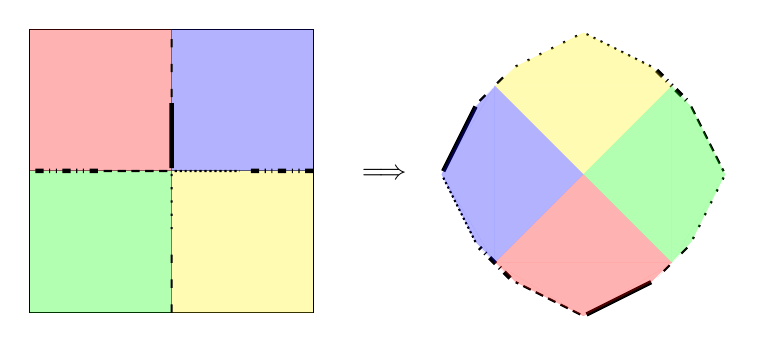
\begin{tikzpicture}[main/.style = {draw, circle, fill=white}]

\begin{scope}[scale=0.3, every node/.append style={transform shape}]
\draw[draw=black] (0, 0) rectangle (12, 12);

\draw[fill=blue, opacity=0.3] (6, 6) rectangle (12, 12);
\draw[fill=yellow, opacity=0.3] (6, 0) rectangle (12, 6);
\draw[fill=green, opacity=0.3] (0, 0) rectangle (6, 6);
\draw[fill=red, opacity=0.3] (0, 6) rectangle (6, 12);

\node[] (A1) at (3, 6) {};
\node[] (A2) at (6, 6) {};
\node[] (A3) at (9, 6) {};

\node[] (B1) at (6, 9){};
\node[] (B3) at (6, 3) {};

\draw[densely dashed, thick] (A1) -- (A2);
\draw[densely dotted, thick] (A2) -- (A3);
\draw[ultra thick] (B1) -- (A2);
\draw[loosely dotted, thick] (A2) -- (B3);
\draw[dashdotdotted, ultra thick] (A1) -- (0, 6);
\draw[dashdotdotted, ultra thick] (12, 6) -- (A3);
\draw[loosely dashed, thick] (B1) -- (6, 12);
\draw[loosely dashed, thick] (6, 0) -- (B3);




\end{scope}

\node () at (4.5, 1.75) {$\implies$};

\begin{scope}[xshift=200,yshift=50, scale=0.45, every node/.append style={transform shape}]
\VertexInv[x=0, y=4]{A1}
\VertexInv[x=2, y=3]{B1}
\VertexInv[x=3, y=2]{C1}
\VertexInv[x=4, y=0]{A2}
\VertexInv[x=3, y=-2]{E1}
\VertexInv[x=2, y=-3]{D1}
\VertexInv[x=0, y=-4]{A3}
\VertexInv[x=-2, y=-3]{C2}
\VertexInv[x=-3, y=-2]{B2}
\VertexInv[x=-4, y=0]{A4}
\VertexInv[x=-3, y=2]{D2}
\VertexInv[x=-2, y=3]{E2}

\VertexInv[x=2.5, y=2.5]{X1}
\VertexInv[x=2.5, y=-2.5]{X2}
\VertexInv[x=-2.5, y=-2.5]{X3}
\VertexInv[x=-2.5, y=2.5]{X4}


\draw [dotted, thick] (A1) -- (B1);
\draw [dashdotdotted, ultra thick] (B1) -- (C1);
\draw [densely dashed, thick] (C1) -- (A2);
\draw [loosely dotted, thick] (A2) -- (E1);
\draw [loosely dashed, thick] (E1) -- (D1);
\draw [ultra thick] (D1) -- (A3);
\draw [densely dashed, thick] (A3) -- (C2);
\draw [dashdotted, ultra thick] (C2) -- (B2);
\draw [densely dotted, thick] (B2) -- (A4);
\draw [ultra thick] (A4) -- (D2);
\draw [loosely dashed, thick] (D2) -- (E2);
\draw [loosely dotted, thick] (E2) -- (A1);

\fill[yellow, opacity=0.3] (-2.5, 2.5) -- (2.5,2.5) -- (0,0) -- (-2.5,2.5);
\fill[yellow, opacity=0.3] (X4) -- (E2) -- (0,4) -- (X4);
\fill[yellow, opacity=0.3] (X1) -- (B1) -- (0,4) -- (X1);
\fill[yellow, opacity=0.3] (-2.5,2.5) -- (2.5,2.5) -- (0,4) -- (-2.5,2.5);

\fill[green, opacity=0.3] (2.5, 2.5) -- (2.5,-2.5) -- (0,0) -- (2.5,2.5);
\fill[green, opacity=0.3] (X1) -- (C1) -- (4,0) -- (X1);
\fill[green, opacity=0.3] (X2) -- (E1) -- (4,0) -- (X2);
\fill[green, opacity=0.3] (2.5,2.5) -- (2.5,-2.5) -- (4,0) -- (2.5,2.5);

\fill[red, opacity=0.3] (-2.5, -2.5) -- (2.5,-2.5) -- (0,0) -- (-2.5,-2.5);
\fill[red, opacity=0.3] (X2) -- (D1) -- (0,-4) -- (X2);
\fill[red, opacity=0.3] (X3) -- (C2) -- (0,-4) -- (X3);
\fill[red, opacity=0.3] (-2.5,-2.5) -- (2.5,-2.5) -- (0,-4) -- (-2.5,-2.5);

\fill[blue, opacity=0.3] (-2.5, -2.5) -- (-2.5,2.5) -- (0,0) -- (-2.5,-2.5);
\fill[blue, opacity=0.3] (X3) -- (B2) -- (-4,0) -- (X3);
\fill[blue, opacity=0.3] (X4) -- (D2) -- (-4,0) -- (X4);
\fill[blue, opacity=0.3] (-2.5,-2.5) -- (-2.5,2.5) -- (-4,0) -- (-2.5,-2.5);


\end{scope}




\end{tikzpicture}
\caption{Cutting the torus into the plane.}
\end{figure}

The idea here is again that we can use this to get critical planar graphs from critical graphs
on the torus, but now we get a cycle-canvas instead of a prism-canvas. See Figure \ref{fig:k6_cyclecanvas} for an example again with $K_6$.

\begin{figure}
\label{fig:k6_cyclecanvas}
\centering
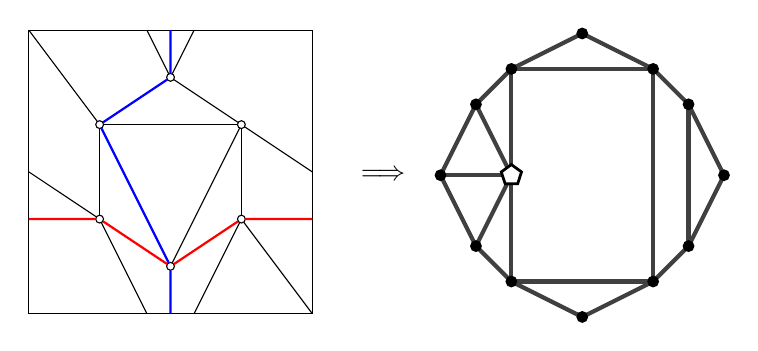
\begin{tikzpicture}[main/.style = {draw, circle, fill=white}]

\begin{scope}[scale=0.3, every node/.append style={transform shape}]
\draw[draw=black] (0, 0) rectangle (12, 12);

\node[main] (A1) at (6, 10) {};
\node[main] (A2) at (3, 4) {};
\node[main] (A3) at (9, 4) {};

\node[main] (B1) at (6, 2){};
\node[main] (B2) at (9, 8) {};
\node[main] (B3) at (3, 8) {};


\draw (A1) -- (B2);
\draw (B2) -- (A3);
\draw [red,thick] (A3) -- (B1);
\draw [red,thick] (B1) -- (A2);
\draw (A2) -- (B3);
\draw [blue,thick](B3) -- (A1);

\draw [blue,thick](A1) -- (6, 12);
\draw [blue,thick](6, 0) -- (B1);
%\draw (A2) -- (0, 0);
%\draw (12, 12) -- (B2);
\draw (A3) -- (12, 0);
\draw (0, 12) -- (B3);

\draw (A2) -- (0, 6);
\draw (12, 6) -- (B2);

\draw (B1) -- (B2);
\draw (B2) -- (B3);
\draw [blue,thick](B3) -- (B1);

\draw [red,thick] (A2) -- (0, 4);
\draw [red,thick](12, 4) -- (A3);
\draw (A2) -- (5, 0);
\draw (5, 12) -- (A1);
\draw (A3) -- (7, 0);
\draw (7, 12) -- (A1);


\end{scope}

\node () at (4.5, 1.75) {$\implies$};

\begin{scope}[xshift=200,yshift=50, scale=0.45, every node/.append style={transform shape}]
\VertexI[x=0, y=4]{A1}
\VertexI[x=2, y=3]{B1}
\VertexI[x=3, y=2]{C1}
\VertexI[x=4, y=0]{A2}
\VertexI[x=3, y=-2]{E1}
\VertexI[x=2, y=-3]{D1}
\VertexI[x=0, y=-4]{A3}
\VertexI[x=-2, y=-3]{C2}
\VertexI[x=-3, y=-2]{B2}
\VertexI[x=-4, y=0]{A4}
\VertexI[x=-3, y=2]{D2}
\VertexI[x=-2, y=3]{E2}

\VertexV[x=-2, y=0]{F}

\Edge(A1)(B1)
\Edge(B1)(C1)
\Edge(C1)(A2)
\Edge(A2)(E1)
\Edge(E1)(D1)
\Edge(D1)(A3)
\Edge(A3)(C2)
\Edge(C2)(B2)
\Edge(B2)(A4)
\Edge(A4)(D2)
\Edge(D2)(E2)
\Edge(E2)(A1)

\Edge(E2)(B1)
\Edge(B1)(D1)
\Edge(C1)(E1)
\Edge(D1)(C2)
\Edge(F)(C2)
\Edge(F)(B2)
\Edge(F)(A4)
\Edge(F)(D2)
\Edge(F)(E2)

\end{scope}
\end{tikzpicture}
\caption{Cutting $K_6$ into a critical cycle-canvas.}
\end{figure}

\begin{observation}
Let $G$ be a $L$-critical graph embedded on the torus with $L$ a $5$-list-assignment,
and let $G'$ be the corresponding planar graph resulting from this procedure with outer face $C$
corresponding to the two cycles we cut through. Then $(G', C, L)$ is a critical cycle-canvas.
\end{observation}

\begin{proof}
Similar argument to the previous observation.
\end{proof}

If the cycles we cut through have lengths $a$ and $b$, the resulting cycle-canvas has cycle length
$2(a+b)$. This gives a bound for the sizes of $6$-list-critical graphs in terms of the sizes of 
their non-contractible cycles via Theorem \ref{linearboundcycletheorem}. However, here the more
interesting idea is the possibility of running the process backwards: that is, of generating
candidates for $6$-list-critical graphs from critical cycle-canvases. 
That is because, as we will see, we have a procedure for the generation of all critical
cycle-canvases by computer. 


\subsection{Our Plan for Graphs With a Non-Contractible Triangle}



Using the above two constructions, we can already devise a plan for finding all $6$-list-critical 
graphs on the torus which have at least one non-contractible triangle.

\begin{enumerate}
	\item Generate all critical cycle-canvases with small cycle sizes (ideally at least up to 
	size $14$ or, better yet, $16$). Also, depending on the approach followed in the next step, it will also be 
	necessary to generate small critical path-canvases or other kinds of critical graphs. 
	\item Prove Conjecture \ref{twotriangleconjecture}. Here, we will try to take advantage
	of the computer-generated graphs in order to obtain the tightest possible bound instead of
	Postle's loose bound.
	\item By cutting through the non-contractible triangle of any $6$-list-critical graph, we
	obtain a critical prism-canvas, and therefore we can reconstruct all possible candidates
	from either the list of all critical prism-canvases (if we obtained such a list from the
	previous step) or a list of all critical cycle-canvases of size $\leq 16$ (by cutting 
	across the non-contractible triangle and the other non-contractible cycle of length 
	$\leq 5$ corresponding to the shortest path between the two precolored triangles in the
	prism-canvas).
\end{enumerate}

This plan only works for $6$-list-critical graphs with edge-width $3$, which is the case for 
the $6$-critical graphs for the previous section. We don't expect to have additional $6$-list-
critical graphs with larger edge-width, especially given (REF POSTLE RESULT EDGEWIDTH), so our
hope would be to find an argument independent of this plan to prove that any $6$-list-critical
graph on the torus must have a non-contractible triangle. 

\todo{check that I defined edge-width and given the result of Postle for ew}

\todo{references for chapters}

The rest of this thesis will be dedicated to describe how to carry out this plan. 
For the first step, we will explain how to perform the computer generation of such critical graphs
in Chapters 3 and 4. Chapter 3 will be about the computer representation of the canvases 	
and the algorithms used for the generation of candidates to be critical canvases, while 
Chapter 4 will be on how to test that such candidates are indeed critical. The techniques 
explained in Chapters 3 and 4 will be applicable not only to cycle-canvases but also to other
types of canvases or graphs with prescribed list sizes more generally. 

For the second step, in Chapter 5 we will explain different approaches to proving Conjecture 
\ref{twotriangleconjecture} using the computer-generated graphs. As of the writing of this thesis,
we have not been able find a proof of this results, because there have been computational and
conceptual obstacles in the approaches we have tried. We will also discuss those setbacks.

Finally, in Chapter 6 we will summarize the computational results obtained by the implementation
of the ideas discussed in the previous chapters and we will expose the partial results we 
have been able to obtain with respect to the third step of the plan. 



 


\chapter{Generation of Critical Graphs}

In this chapter we describe algorithms for processing and generating critical canvases via computer search.

\section{Representation of Canvases}

The first step is deciding how to represent canvases in our algorithms. Recall that a canvas $T$ is a tuple 
$(G, S, L)$ where $G$ is a plane graph, $S$ is a subgraph of the outer face and $L$ is a list assignment for 
$G$ satisfying some conditions. Here, in each algorithm we will usually be working with one particular family of 
canvases at a time, for example cycle-canvases or path-canvases with a fixed size of cycle or path, so the 
information about the subgraph $S$ can be ``implicit'' in each different representation for each different algorithm
instead of working with a general representation that allows all canvases. Also, in some scenarios we will be 
working with conditions on the list assignment $L$ which are different from the ones in the definition of canvas.
In this section we intend to just expose some general ideas about how the representation of graphs in this context
can be done, which will be afterwards applied in different scenarios.

The most important thing to state is that we will not be interested in storing the list assignment $L$ at all. 
This is because there is a significant combinatorial explosion in the number of list assignments to be considered and
we are interested in the graphs themselves, not the list assignments. Also, most of the results
we will be using such as Lemma \ref{gluinglemma} or Theorem \ref{cyclechordtripodtheorem} are directly related to subgraphs
and not list assignments, and while they are in theory stated with respect to a fixed list assignment, it is more
useful in practice to not consider the list assignment at all. 

Thus, when we generate all critical canvases $(G, S, L)$, what we will actually be doing is generate all pairs $(G, S)$ 
such that there exists some list assignment $L$  so that $(G, S, L)$ is a critical canvas. In some scenarios, we will also
be interested in storing the prescribed size of the list assignment for each vertex: that is, we will be storing a tuple $(G, S, f)$
with $f : V(G) \rightarrow \mathbb{N}$ so that we will only be considering list assignments $L$ with $|L(v)| = f(v)$, but other
than that we will not store information about the actual list assignment. 

We store the information of the graph $G$ with an adjacency list. We will also be interested in storing the planar embedding of the graph:
to do so, we order the edges in the adjacency list of each vertex according to their clockwise order in the embedding (as in a
\emph{rotation system}). This information, together with the information of which vertices are in the outer face, is enough to reconstruct
the embedding. 

We will want to test when two canvases are isomorphic. More generally, we will want to have a canonical form for each canvas, so that
given a set of canvases $\mathcal{S}$ and a new canvas $T$, we can check whether there is a canvas isomorphic to $T$ in $\mathcal{S}$ by checking the 
presence of the corresponding canonical form of $T$ in an associative array with the canonical forms of the canvases in $\mathcal{S}$.

In order to produce the canonical form, define the \emph{transcript of the DFS traversal starting at edge $u \rightarrow v$} as the string generated by procedure
dfsTranscript in Algorithm \ref{alg:canonization}. That is, we do a depth-first traversal of the graph following the edges on each vertex in clockwise order, assigning labels to vertices based in the
order in which we first visit them and storing information for each edge we visit in the traversal: \texttt{F} for edges towards a new vertex in the traversal,
\texttt{B} for edges towards the immediately previous vertex in the traversal stack (which signifies the end of the edges for the current vertex and the return
to the previous vertex of the stack) and the label of the other endpoint for other edges. See Algorithm \ref{alg:canonization} for details.

\begin{algorithm}
\caption{Canonization of Plane Graphs.}
\label{alg:canonization}
\SetAlgoLined
\SetKwComment{Comment}{/* }{ */}
\SetKwProg{Fn}{function}{}{end}

\Comment*[h]{Returns lexicographically smallest DFS Transcript}
\Fn{canonicalForm($G$)}{ 
	$s \gets \text{``\#''}$\;
	\For{$uv \text{ in outer face of } G$} {
		$t \gets \text{dfsTranscript}(G, u, v)$\;
		\If{$t <_{\ell} s$} {
			$s \gets t$\;
		}
	}
	return $s$\;
}
\Fn{dfsTranscript($G$, $u$, $v$)} {
	$s \gets \text{``''}$\;
	$A \gets \text{array}(|V(G)|)$\;
	$A[u] \gets \text{firstIdentifier}()$\;
	\Comment*[r]{$A$ is the array that stores identifiers of already visited vertices, initially initialized with $\emptyset$ for all vertices}
	\For {$w \text{ neighbor of } u \text{ in clockwise order starting with } v$}{
		dfs($G$, $w$, $u$, $s$, $A$)\;
	}
	return $s$\;
}
\Fn{dfs($G$, $u$, $p$, $s$, $A$)} {
	\If {$A[u] \neq \emptyset$} {
		$s \gets s + A[u]$\;
		return\;
	}
	$A[u] \gets \text{nextIdentifier}()$\;
	$s \gets s + \text{`F'}$\;
	\For {$v \neq p \text{ neighbor of } u \text{ in clockwise order starting in the next neighbor after } p$}{
		dfs($G$, $v$, $u$, $s$, $A$)\;
	}
	$s \gets s + \text{`B'}$\;
}


\end{algorithm}


\begin{figure}
\centering
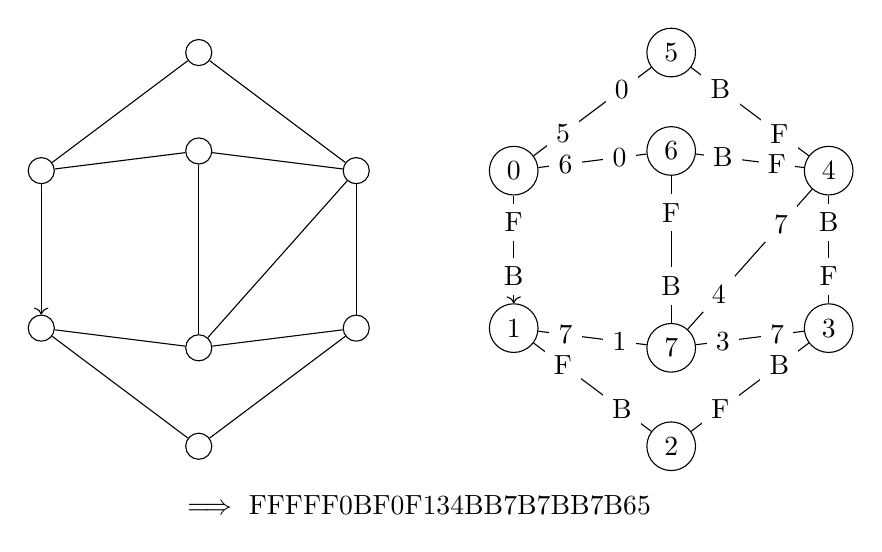
\begin{tikzpicture}[main/.style = {draw, circle, fill=white}]

		\node[main] (0) at (-2, 2) {};
		\node[main] (1) at (-2, 0) {};
		\node[main] (2) at (0, -1.5) {};
		\node[main] (3) at (2, 0) {};
		\node[main] (4) at (2, 2) {};
		\node[main] (5) at (0, 3.5) {};
		\node[main] (6) at (0, 2.25) {};
		\node[main] (7) at (0, -0.25) {};
		
		\draw[->] (0) -- (1);
		\draw (1) -- (2) ;
		\draw (2) -- (3) ;
		\draw (3) -- (4) ;
		\draw (4) -- (5) ;
		\draw (5) -- (0) ;
		\draw (4) -- (6) ;
		\draw (6) -- (0) ;
		\draw (6) -- (7) ;
		\draw (7) -- (1) ;
		\draw (7) -- (3) ;
		\draw (7) -- (4) ;
		
		
		
	
	
		\node[main] (0A) at (4, 2) {0};
		\node[main] (1A) at (4, 0) {1};
		\node[main] (2A) at (6, -1.5) {2};
		\node[main] (3A) at (8, 0) {3};
		\node[main] (4A) at (8, 2) {4};
		\node[main] (5A) at (6, 3.5) {5};
		\node[main] (6A) at (6, 2.25) {6};
		\node[main] (7A) at (6, -0.25) {7};
		
		\draw[->] (0A) -- (1A) node [near start, fill=white] {F} node [near end, fill=white] {B};
		\draw (1A) -- (2A) node [near start, fill=white] {F} node [near end, fill=white] {B};
		\draw (2A) -- (3A) node [near start, fill=white] {F} node [near end, fill=white] {B};
		\draw (3A) -- (4A) node [near start, fill=white] {F} node [near end, fill=white] {B};
		\draw (4A) -- (5A) node [near start, fill=white] {F} node [near end, fill=white] {B};
		\draw (5A) -- (0A) node [near start, fill=white] {0} node [near end, fill=white] {5};
		\draw (4A) -- (6A) node [near start, fill=white] {F} node [near end, fill=white] {B};
		\draw (6A) -- (0A) node [near start, fill=white] {0} node [near end, fill=white] {6};
		\draw (6A) -- (7A) node [near start, fill=white] {F} node [near end, fill=white] {B};
		\draw (7A) -- (1A) node [near start, fill=white] {1} node [near end, fill=white] {7};
		\draw (7A) -- (3A) node [near start, fill=white] {3} node [near end, fill=white] {7};
		\draw (7A) -- (4A) node [near start, fill=white] {4} node [near end, fill=white] {7};
		
		
		\node[] at (2.75, -2.25) {$\implies$ FFFFF0BF0F134BB7B7BB7B65};

\end{tikzpicture}
\caption{Example of a DFS traversal transcript for a graph. It is the lexicographically smallest transcript in this case.}
\end{figure}


We compute such string for all the edges of the outer face as starting edges, and we take the lexicographically smallest one as the canonical form. It is clear that
two plane graphs have the same canonical string if and only if they have isomorphic (in terms of the rotation system) embeddings. 


\section{Generation of Critical Cycle-Canvases}

Our algorithm for the generation of critical cycle-canvases is based on Theorem \ref{cyclechordtripodtheorem}. 
This theorem says that every critical cycle-canvas can either be decomposed into two smaller critical 
cycle-canvases through a chord in the outer face, it can be decomposed into a ``tripod'', a vertex $v$ 
with at least $3$ neighbors in $C$, and a smaller critical cycle-canvas contained in the only nonempty 
face incident with $v$. In these decompositions, it is possible that instead of a smaller critical canvas 
we get an empty canvas, which is technically not critical. 

This implies that we can generate all critical cycle-canvases from smaller cycle-canvases by gluing
cycle-canvases through outer face edges to get a canvas with a chord, or by adding a tripod to the
outside of a cycle-canvas. We then have to check whether the resulting canvas is indeed critical,
since the decomposition into two smaller critical cycle-canvases is a necessary but not sufficient condition
for criticality. We will see how to do this in Chapter 4.



If we are generating cycle-canvases with cycle length $\ell$, then a chord partitions
the cycle-canvas into two cycle-canvases of length $a$, $b$ with $a, b \geq 3$ and $a + b = \ell + 2$, so 
$a, b \leq \ell-1$ and therefore if we have generated all cycle-canvases with cycle length $< \ell$ we can generate
all cycle-canvases with cycle length $\ell$ with a chord. In the case of adding a tripod, though, if the vertex $v$ of
the tripod is adjacent to only three adjacent vertices in the outer face, then the smaller cycle-canvas has the same
cycle length as the larger cycle-canvas.

In order to resolve this, what we do is first generate all the cycle-canvases obtained from cycle-canvases with smaller cycle size, enqueue the resulting critical canvases, and then process the canvases from the queue and add tripods 
to three consecutive vertices in all possible ways, enqueueing the new critical cycle-canvases that are found. See Algorithm \ref{alg:cyclecanvases} for a detailed
description.


\begin{algorithm}
\small
\caption{Generation of Critical Cycle-Canvases.}
\label{alg:cyclecanvases}
\SetAlgoLined
\SetKwComment{Comment}{/* }{ */}
\SetKwProg{Fn}{function}{}{end}
\Comment*[h]{Generate critical canvases of cycle size $\ell$, including empty one}

\Fn{generateCriticalCycleCanvases($\ell$)}{ 
	
	\For{$i = 3, \ldots, \ell-1$} {
		$S_i \gets \text{generateCriticalCycleCanvases}(i)$\;
	}
	$S \gets \{ \text{emptyCycle}(\ell) \}$\;
	
	\For{$a = 3, \ldots, \ell-1$} {
		$b \gets \ell-a+2$\;
		\For{$G_1 \in S_a$} {
			\For{$G_2 \in S_b$} {
				$T \gets \text{fuseChordSet}(G_1, G_2)$\; 
				\Comment*[r]{Set of cycle-canvases obtained by fusing $G_1$ and $G_2$ along outer cycle edges in all possible ways}
				\For{$G \in T$} {
					\If{$G \not\in S$ AND $\text{isCritical}(G)$} {	
						$S \gets S \cup \{G\}$\;
					}
				} 
			}
		}
	}
	\For{$k = 3, \ldots, \ell-1$} {
		\For{$G_1 \in S_k$} {
			$T \gets \text{addTripodSet}(G_1, \ell-k+3, 3)$\;
			\Comment*[r]{Set of cycle-canvases obtained by adding a tripod with $3$ neighbors in the outer face to get a cycle-canvas of length $\ell$ in all possible ways}
			\For{$G \in T$} {
				\If{$G \not\in S$ AND $\text{isCritical}(G)$} {	
					$S \gets S \cup \{G\}$\;
				}
			} 
		}
	}	
	$Q \gets \text{Queue}(S)$\; 
	\While{$Q \text{ is not empty}$} {
		$G_1 \gets \text{first}(Q)$\;
		$\text{dequeue}(Q)$\;
		$T \gets \text{addTripodSet}(G_1, 3, 3)$\;
		\For{$G \in T$} {
			\If{$G \not\in S$ AND $\text{isCritical}(G)$} {	
				$S \gets S \cup \{G\}$\;
				$\text{enqueue}(Q, G)$\;
			}
		} 
	}
	return $S$\;
}


\end{algorithm}



Note that we only need to add tripods with $3$ adjacent neighbors since vertices with a larger number of neighbors in the
outer face can be obtained by first adding chords and then adding finally adding a tripod with $3$ neighbors. However, 
often we are interested in just generating chordless critical canvases. In that case, we do need to add tripods of all sizes.
The modified algorithm for chordless critical cycle-canvases is Algorithm \ref{alg:chordlesscyclecanvases}.

\begin{algorithm}
\caption{Generation of Chordless Critical Cycle-Canvases.}
\label{alg:chordlesscyclecanvases}
\SetAlgoLined
\SetKwComment{Comment}{/* }{ */}
\SetKwProg{Fn}{function}{}{end}
\Comment*[h]{Generate chordless critical canvases of cycle size $\ell$, including empty one}

\Fn{generateChordlessCriticalCycleCanvases($\ell$)}{ 
	
	\For{$i = 3, \ldots, \ell-1$} {
		$S_i \gets \text{generateChordlessCriticalCycleCanvases}(i)$\;
	}
	$S \gets \{ \text{emptyCycle}(\ell) \}$\;
	\For{$k = 3, \ldots, \ell-1$} {
		\For{$j = 3, \ldots, \ell-k+3$} {
			\For{$G_1 \in S_k$} {
				$T \gets \text{addTripodSet}(G_1, \ell-k+3, j)$\;
				\For{$G \in T$} {
					\If{$G \not\in S$ AND $\text{isCritical}(G)$} {	
						$S \gets S \cup \{G\}$\;
					}
				} 
			}
		}
	}	
	$Q \gets \text{Queue}(S)$\; 
	\While{$Q \text{ is not empty}$} {
		$G_1 \gets \text{first}(Q)$\;
		$\text{dequeue}(Q)$\;
		$T \gets \text{addTripodSet}(G_1, 3, 3)$\;
		\For{$G \in T$} {
			\If{$G \not\in S$ AND $\text{isCritical}(G)$} {	
				$S \gets S \cup \{G\}$\;
				$\text{enqueue}(Q, G)$\;
			}
		} 
	}
	return $S$\;
}


\end{algorithm}


\section{Generation of Critical Wedges}
\label{sec:generationwedges}

We are will be not only interested in generating critical cycle-canvases, but also critical path-canvases or wedges. 
There are infinitely many of those for path length greater than $1$, but as we will see in coming sections, 
we will be able to have a finite number of them if we impose additional conditions. 

Fortunately, we also have an analogue of Theorem \ref{cyclechordtripodtheorem} for wedges:

\begin{theorem}[Wedge Chord or Tripod Theorem]
If $(G, P, L)$ is a $2$-connected critical wedge, then either

\begin{enumerate}
\item The outer walk $C$ has a chord in $G$, or
\item there exists a vertex $v \in V(G) \setminus V(P)$ with at least three neighbors on $P$ such that at most one of the faces of 
$G[\{v\} \cup V(P)]$ includes a vertex or edge of $G$. 
\end{enumerate}
\end{theorem}

\begin{proof}
Assume not. Then, we will show that every $L$-coloring of $P$ extends to an $L$-coloring of $G$, contradiction. Let $\phi$ be any $L$-coloring of $P$, 
$G' = G \setminus P$ and $L'(v) = L(v) \setminus \{\phi(u) : u \in V(P) \text{ neighbor of } v \}$ for each $v \in V(G')$. 
Note that $|L'(v)| \geq 5$ for every interior vertex of $G'$. Let $C'$ be the outer walk of $G'$ and let $v_1$, $v_2$ be the two vertices of 
$G'$ that were adjacent to the two endpoints of $P$ in $G$. Note that $|L'(v)| \geq 3$ for all $v \in C' \setminus \{v_1, v_2\}$ since 
$G$ was $2$-connected and had no chords, and $|L(v_1)|, |L(v_2)| \geq 2$. Hence, $G'$ is $L'$-colorable by Theorem \ref{twolistsofsizetwo}.
\end{proof}

(This version of the theorem is slightly different than the one proved by Postle in \cite{postlethesis}).

Based on this theorem, we can design an algorithm to generate critical wedges similar to the one used to generate critical canvases.  
The main additional considerations we need to take into account are:

\begin{itemize}
	\item We have to generate non-$2$-connected critical wedges by gluing smaller critical wedges along the cutvertices.
	 Observe that the cutvertices must necessarily be part of $P$.
	\item Now adding a chord whose endpoint is the vertex next to the endpoints of the precolored path produces a wedge
	with the same path length, so we need to add those chords in the part of the algorithm using a queue.
	\item Chords with one endpoint in the precolored path and another endpoint outside the precolored path
	need to be treated separately from chords with two endpoints in the precolored path.
	Note that it is not possible to have a chord with two endpoints outside the precolored path (or one endpoint
	in an endpoint in the precolored path) because of Theorem \ref{thomassenstrongertheorem}.
\end{itemize}


\begin{algorithm}
\caption{Generation of Critical Wedges.}
\SetAlgoLined
\SetKwComment{Comment}{/* }{ */}
\SetKwProg{Fn}{function}{}{end}
\Comment*[h]{Generate critical wedges of path size $\ell$, assuming
those of path size $< \ell$ have been already generated and are stored
in variable $W_i$, and the biconnected ones are in $B_i$.}
\Fn{generateCriticalWedges($\ell$)}{ 
	$B_\ell \gets \text{generateBiconnectedCriticalWedges}(\ell)$\; 			
	$W_\ell \gets B_\ell \cup \text{generateNonBiconnectedCriticalWedges}(\ell)$\;
}

\Fn{generateBiconnectedCriticalWedges($\ell$)}{
	$S \gets \text{emptyCycle}(\ell) \cup \text{wedgesFromPathChords}(\ell) \cup \text{wedgesFromNonPathChords}(\ell) \cup \text{wedgesFromTripods}(\ell)$\;
	$Q \gets \text{Queue}(S)$\; 
	\While{$Q \text{ is not empty}$} {
		$G_1 \gets \text{first}(Q)$\;
		$\text{dequeue}(Q)$\;
		$T \gets \text{addTripodSet}(G_1, 3, 3)$\;
		$T \gets T \cup \text{addSizeTwoWedgesInEndpointsSet}(G_1)$\;
		\Comment*[r]{Set of wedges obtained by fusing wedges of size two
		in the endpoints of wedge $G_1$ in all possible ways}
		\For{$G \in T$} {
			\If{$G \not\in S$ AND $\text{isCritical}(G)$} {	
				$S \gets S \cup \{G\}$\;
				$\text{enqueue}(Q, G)$\;
			}
		} 
	}
	return $S$\;
}

\Fn{generateNonBiconnectedCriticalWedges($\ell$)}{
	$S \gets \text{emptyPath}(\ell)$\;
	\For{$a = 2, \ldots, \ell-2$} {
		$b \gets \ell-a$\;
		\For{$G_1 \in W_a$} {
			\For{$G_2 \in W_b$} {
				$G \gets \text{fuseEndpoints}(G_1, G_2)$\;
				\If{$G \not\in S$ AND $\text{isCritical}(G)$} {	
					$S \gets S \cup \{G\}$\;
				}
			}
		}
	}
	
	return $S$\;
}


\end{algorithm}

\begin{algorithm}
\footnotesize
\caption{Functions Generating Critical Wedges from Smaller Path Lengths}
\SetAlgoLined
\SetKwComment{Comment}{/* }{ */}
\SetKwProg{Fn}{function}{}{end}

\Fn{wedgesFromPathChords($\ell$)}{ 
	$S \gets \{\}$\;
	\For{$a = 2, \ldots, \ell-1$} {
		\For{$G' \in B_a$} {
			$T \gets \text{extendPathChordSet}(G', \ell-a)$\;
			\Comment*[r]{Set of wedges obtained by adding $\ell-a$ consecutive new precolored vertices between two adjacent precolored vertices of $G'$, making the previous edge of $G'$ a chord in the path.}
			\For{$G \in T$} {
				\If{$G \not\in S$ AND $\text{isCritical}(G)$} {	
					$S \gets S \cup \{G\}$\;
				}
			}
		}
	}
	return $S$\;
}

\Fn{wedgesFromNonPathChords($\ell$)}{
	$S \gets \{\}$\;
	\For{$a = 4, \ldots, \ell-1$} {
		$b \gets \ell-a+3$\;
		\For{$G_1 \in B_a$} {
			\For{$G_2 \in B_b$} {
				$T = \text{fuseChordSet}(G_1, G_2)$\;
				\For{$G \in T$} {
					\If{$G \not\in S$ AND $\text{isCritical}(G)$} {	
						$S \gets S \cup \{G\}$\;
					}
				}
			}
		}
	}
	
	return $S$\;
}

\Fn{wedgesFromTripods($\ell$)}{
	$S \gets \{\}$\;
	\For{$k = 3, \ldots, \ell-1$} {
		\For{$j = 3, \ldots, \ell-k+3$} {
			\For{$G' \in B_k$} {
				$T \gets \text{addTripodSet}(G', \ell-k+3, j)$\;
				\For{$G \in T$} {
					\If{$G \not\in S$ AND $\text{isCritical}(G)$} {	
						$S \gets S \cup \{G\}$\;
					}
				} 
			}
		}
	}	
	return $S$\;
}


\end{algorithm}



\chapter{Criticality Testing}

In this chapter we describe algorithms used to determine list-criticality of graphs. Recall that we are 
not storing the explicit list assignment $L$ for our graphs, so what we want to check is whether there 
exists a $L$ so that the graph is critical with respect to that $L$. However, even if $L$ was fixed, 
it would still be a computationally hard problem to determine criticality. What we will do instead is check 
for weaker properties, and therefore admit some false positives, that is, some graphs we identify as list-critical 
for which actually no suitable $L$ exist. Our hope is that the tests will be exhaustive enough so that finiteness 
results such as \ref{linearboundcycletheorem} still hold for the weaker properties we are testing, and our algorithms 
terminate. We will see that indeed, the algorithms described here work very well in practice at discarding non-critical graphs. 

\todo{explain that we work with graphs with prescribed list sizes}

\section{Degree Properties}

We can start with an easy observation:

\begin{observation}
\label{degreeobs}
In a $f$-list-critical graph, $d(v) \geq f(v)$ for all vertices $v$.
\end{observation}

So if we find a vertex with degree less than the prescribed list size, we can conclude that the graph is not list-critical. 
However, this is a very weak test. We can incorporate another test concerning the vertices with $d(v) = |L(v)|$: there is
the following result by Gallai showing that the subgraph induced by those vertices must have a certain structure, generalizing 
the classical Brooks theorem for vertex coloring:

\begin{theorem}[Gallai \cite{gallaikritische}]
Let $G$ be a $f$-list-critical graph and let $H$ be the subgraph
of $H$ induced by the vertices with $d(v) = f(v)$. 
Then each $2$-connected component of $H$ is a complete graph or an odd cycle.
\end{theorem}

\section{Reducible Configurations}

The \emph{method of reducible configurations} is a usual technique in graph coloring problems. It consists in identifying subgraphs 
or other structures that can not appear in critical graphs. We have the following observation:

\begin{proposition}
\label{reduciblecolorableprop}
Let $G$ be an $f$-list-critical graph, and let $H$ be an induced subgraph of $G$ such that $\forall v \in H, f(v) > d_{G\setminus H}(v)$,
where $d_{G \setminus H}(v)$ is the number of neighbors of $v$ which are not in $H$. Then $H$ is not $g$-list-colorable, where $g(v) = f(v) -d_{G\setminus H}(v)$.
\end{proposition}

\begin{proof}
If $G = H$, it is immediate. Assume $H \subsetneq G$, and let $G$ be $L$-critical. 
Let $\phi$ be a coloring of $G \setminus H$, and let $L'$ be the $g$-list-assignment of $H$ given by 
$L'(v) = L(v) \setminus \{\phi(u) : u \in N_G(v), u \not\in H\}$. 
Then $H$ is not $L'$-colorable: since otherwise, the $L$-coloring $\phi$ of $G \setminus H$ would extend to $G$, contradiction.
\end{proof}

\begin{figure}
\centering
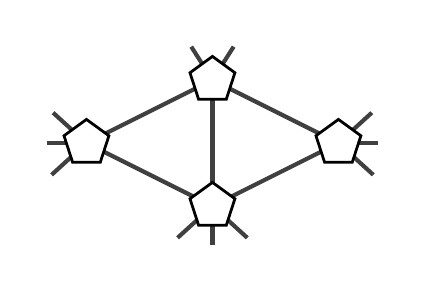
\begin{tikzpicture}[scale=0.8]
\VertexV[y=1]{A}
	\VertexV[x=-2]{B}
	\VertexV[y=-1]{C}
	\VertexV[x=2]{D}
	
	\node[above right = 2.5mm and 0.5mm of A] (A1){};
	\node[above left  = 2.5mm and 0.5mm of A] (A3){};
	
	\node[above left = 2mm and 2.5mm of B] (B1){};
	\node[left = 2.5mm of B] (B2){};
	\node[below left = 2mm and 2.5mm of B] (B3){};
	
	\node[above right = 2mm and 2.5mm of D] (D1){};
	\node[right = 2.5mm of D] (D2){};
	\node[below right = 2mm and 2.5mm of D] (D3){};
	
	\node[below right = 2mm and 2.5mm of C] (C1){};
	\node[below = 2.5mm of C] (C2){};
	\node[below left = 2mm and 2.5mm of C] (C3){};
	
	\Edge(A)(A1)
	\Edge(A)(A3)
	
	\Edge(B)(B1)
	\Edge(B)(B2)
	\Edge(B)(B3)
	
	\Edge(C)(C1)
	\Edge(C)(C2)
	\Edge(C)(C3)
	
	\Edge(D)(D1)
	\Edge(D)(D2)
	\Edge(D)(D3)
		
	\Edge(A)(B)
	\Edge(A)(C)
	\Edge(A)(D)
	\Edge(B)(C)
	\Edge(C)(D)

\end{tikzpicture}
\begin{tikzpicture}
\node[] at (0, 1.3) {$\implies$};
\node[] at (0, 0) {};
\end{tikzpicture}
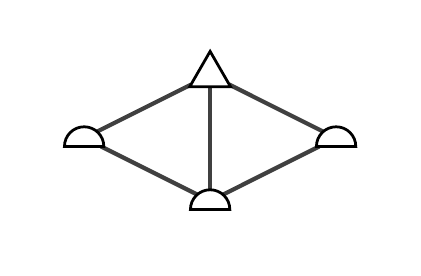
\begin{tikzpicture}[scale=0.8]
\VertexIII[y=1]{A}
	\VertexII[x=-2]{B}
	\VertexII[y=-1]{C}
	\VertexII[x=2]{D}
	
		\node[above right = 2.5mm and 0.5mm of A] (A1){};
	\node[above left  = 2.5mm and 0.5mm of A] (A3){};
	
	\node[above left = 2mm and 2.5mm of B] (B1){};
	\node[left = 2.5mm of B] (B2){};
	\node[below left = 2mm and 2.5mm of B] (B3){};
	
	\node[above right = 2mm and 2.5mm of D] (D1){};
	\node[right = 2.5mm of D] (D2){};
	\node[below right = 2mm and 2.5mm of D] (D3){};
	
	\node[below right = 2mm and 2.5mm of C] (C1){};
	\node[below = 2.5mm of C] (C2){};
	\node[below left = 2mm and 2.5mm of C] (C3){};
	
	\Edge(A)(B)
	\Edge(A)(C)
	\Edge(A)(D)
	\Edge(B)(C)
	\Edge(C)(D)

\end{tikzpicture}
\caption{Illustration of \ref{reducibleobs}: from a subgraph, we get a graph with prescribed list sizes.}
\end{figure}

We can consider \ref{degreeobs} to be a particular case of \ref{reduciblecolorableprop}. 
In \ref{reduciblecolorablefigure} we see a couple of examples of small graphs that are always $f$-colorable,
so one possible test we can add to our criticality testing procedure is to search for occurrences of those graphs as induced subgraphs,
and if one is found then conclude that the graph is not critical.



\begin{figure}

\centering
\begin{subfigure}{0.4\textwidth}
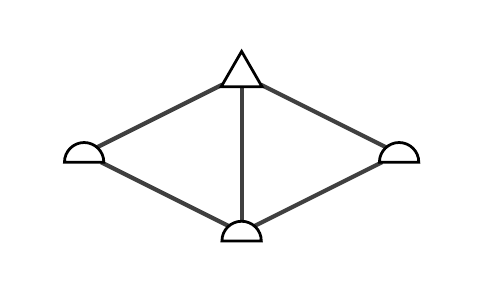
\begin{tikzpicture}
\VertexIII[y=1]{A}
	\VertexII[x=-2]{B}
	\VertexII[y=-1]{C}
	\VertexII[x=2]{D}
	
		\node[above right = 2.5mm and 0.5mm of A] (A1){};
	\node[above left  = 2.5mm and 0.5mm of A] (A3){};
	
	\node[above left = 2mm and 2.5mm of B] (B1){};
	\node[left = 2.5mm of B] (B2){};
	\node[below left = 2mm and 2.5mm of B] (B3){};
	
	\node[above right = 2mm and 2.5mm of D] (D1){};
	\node[right = 2.5mm of D] (D2){};
	\node[below right = 2mm and 2.5mm of D] (D3){};
	
	\node[below right = 2mm and 2.5mm of C] (C1){};
	\node[below = 2.5mm of C] (C2){};
	\node[below left = 2mm and 2.5mm of C] (C3){};
	
	\Edge(A)(B)
	\Edge(A)(C)
	\Edge(A)(D)
	\Edge(B)(C)
	\Edge(C)(D)

\label{fig:reducible1}
\end{tikzpicture}
\end{subfigure}
\begin{subfigure}{0.4\textwidth}
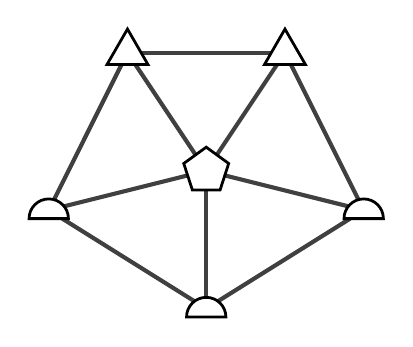
\begin{tikzpicture}
\VertexIII[x=-1,y=2]{A1}
	\VertexIII[x=1,y=2]{A2}
	\VertexII[x=-2]{B1}
	\VertexII[y=-1.25]{B2}
	\VertexII[x=2]{B3}
	\VertexV[y=0.5]{C}
	
	\Edge(C)(A1)
	\Edge(C)(A2)
	\Edge(C)(B1)
	\Edge(C)(B2)
	\Edge(C)(B3)
	\Edge(A1)(A2)
	\Edge(A2)(B3)
	\Edge(B3)(B2)
	\Edge(B2)(B1)
	\Edge(B1)(A1)

\end{tikzpicture}
\label{fig:reducible2}
\end{subfigure}
\caption{Some colorable reducible configurations.}
\label{fig:colorablereducible}
\end{figure}

However, there are also reducible configurations which are not $f$-colorable.

\begin{definition}
A graph $G$ is said to be \emph{$f$-reducible} if there is a proper subgraph $H \subsetneq G$ so that
for all $f$-list-assignments $L$ of $G$, if $H$ is $L_{\restriction_H}$-colorable then $G$ is $L$-colorable. 
\end{definition}

\begin{proposition}
Let $G$ be an $f$-list-critical graph, and let $H$ be an induced subgraph of $G$ such that $\forall v \in H, f(v) > d_{G\setminus H}(v)$,
where $d_{G \setminus H}(v)$ is the number of neighbors of $v$ which are not in $H$. Then $H$ is not $g$-reducible, where $g(v) = f(v) -d_{G\setminus H}(v)$.
\end{proposition}

\begin{proof}
Assume not, and let $H'$ be the corresponding subgraph of $H$ for which all $g$-colorings extend. Let $G$ be $L$-critical. 
There exists an $L$-coloring $\phi$ of $G \setminus (H \setminus H')$. Let $L'$ be the $g$-list-assignment of $H$ given by 
$L'(v) = L(v) \setminus \{\phi(u) : u \in N_G(v), u \not\in H\}$. Note that $\phi_{\restriction_{H'}}$ is an $L'$-coloring of $H'$, so there must
be an $L'$-coloring $\psi$ of $H$. But then the coloring $\Phi$ given by $\Phi(v) = \psi(v)$ for $v \in H$, $\Phi(v) = \phi(v)$ for $v \in G \setminus H$ is 
a $L$-coloring of $G$, contradiction. 
\end{proof}

\begin{figure}

\centering
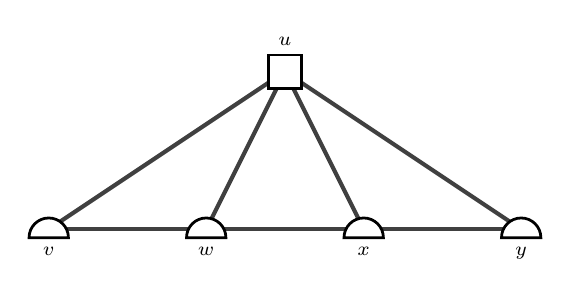
\begin{tikzpicture}
\VertexIV[y=1, label=$u$,position=above]{X}
	\VertexII[x=-3, y=-1, label=$v$, position=below]{A}
	\VertexII[x=-1, y=-1, label=$w$,position=below]{B}
	\VertexII[x=1, y=-1, label=$x$,position=below]{C}
	\VertexII[x=3, y=-1, label=$y$,position=below]{D}
	
	\Edge(X)(A)
	\Edge(X)(B)
	\Edge(X)(C)
	\Edge(X)(D)
	\Edge(A)(B)
	\Edge(B)(C)
	\Edge(C)(D)

\end{tikzpicture}
\caption{A non-colorable reducible configuration.}
\label{fig:noncolorablereducible}
\end{figure}

\begin{observation}
The graph depicted in \ref{fig:noncolorablereducible} with prescribed list sizes $f$ is $f$-reducible.
\end{observation}

\begin{proof}
Let us characterize the $f$-list-assignments $L$ for which the graph is not $L$-colorable. First, note that if $L(v) \neq L(w)$ or $L(x) \neq L(y)$
one can precolor both $w$ and $x$ so that the resulting graph with the corresponding colors removed from the lists is a path with list sizes at least $2$
in all vertices except in one endpoint, with list size at least $1$, so it is colorable. Therefore, we have $L(v) = L(w)$ and $L(x) = L(y)$. Then, note
that $L(v), L(x) \subseteq L(u)$, since otherwise by coloring one vertex with a color not in $L(u)$ one can always color the graph. Therefore, the $f$-list-assignments
for which the graph is not $L$-colorable are those of the form $L(u) = \{A, B, C, D\}$, $L(v) = L(w) = \{A, B\}$, $L(x) = L(y) = \{C, D\}$. But for those list assignments
the graph without edge $wx$ is also not $L$-colorable, so for any $f$-list-assignment $L$ the graph is $L$-colorable if and only if the subgraph without the edge $wx$ is
$L$-colorable.
\end{proof}

\section{The Alon-Tarsi Method}

While checking for the small reducible configurations we found in the previous section is helpful, it is not good enough, because
there are larger graphs which are always $f$-colorable but do not contain any of the reducible configurations. One could augment the
list of configurations to check by manually those graphs when they are encountered, but this is ineffective and also inefficient because
induced subgraph isomorphism testing starts being very expensive with larger subgraphs. 
We would, then, like to have a systematic method to find when graphs with prescribed list sizes $f$ are $f$-list-colorable. Alon and Tarsi
provided a useful criterion:

\begin{theorem}[Alon-Tarsi, \cite{alontarsi}]
\label{alontarsitheorem}
Let $G$ be a directed graph on vertices $v_1, \ldots, v_n$, and let $L$ be an assignment of lists to vertices of $G$ such that 
$|L(v_i)| \geq d^+(v_i)+1$ for $i = 1, \ldots, n$. If $G$ has a different number of even and odd spanning eulerian subgraphs,
then $G$ has an $L$-coloring.
\end{theorem}

\todo{Define directed graphs and d+ either here or in the introduction}.

Here \emph{even} and \emph{odd} eulerian subgraphs refer to the number of edges. We will explain the proof of this theorem here,
since it will give us insight into how to implement it in a more efficient way than enumerating all eulerian subgraphs. For the
proof we will need an algebraic result known as Combinatorial Nullstellensatz.

\begin{theorem}[Combinatorial Nullstellensatz \cite{alonnullstellensatz}]
Let $\mathbb{K}$ be a field and $p(x_1, \ldots, x_n) \in \mathbb{K}[x_1, \ldots, x_n]$ be a nonzero polynomial and let $t_1, \ldots, t_n$ be nonnegative integers such that the
 degree of $p$ is $t_1 + \ldots + t_n$ and the coefficient of $\prod_{i=1}^n x_i^{t_i}$ in $p$ is nonzero. 
 Let $S_1, \ldots, S_n$ be subsets of $\mathbb{K}$ such that $|S_i| \geq t_i+1$. Then there exist $a_1 \in S_1, \ldots, a_n \in S_n$ such that
$p(a_1, \ldots, a_n) \neq 0$.
\end{theorem}

\subsection{Proof of the Alon-Tarsi Theorem}

\begin{definition}
For a directed graph $G$ with $n$ vertices $v_1, \ldots, v_n$, we define its \emph{graph polynomial} $p_G(x_1, \ldots, x_n)$ as:
\begin{equation}
\label{eq:graphpolynomialproduct}
p_G(x_1, \ldots, x_n) = \prod_{\overrightarrow{v_iv_j}\in E(G)} (x_j-x_i).
\end{equation}
\end{definition}


\begin{observation}
If we associate each color with a different number (we work in, say, $\mathbb{C}$), then $\phi$ is a proper coloring of 
$G$ if and only if $p_G(\phi(v_1), \ldots, \phi(v_n)) \neq 0$. 
\end{observation}

\begin{proposition}
\ref{polynomialatproposition}
Let $G$ be as in the hypothesis of the Alon-Tarsi theorem.
If the coefficient of $p_G$ at $\prod_{i=1}^n x_i^{d^+(v_i)}$ is non-zero, then $G$ has an $L$-coloring.
\end{proposition}
\begin{proof}
The total degree of $p_G$ is $|E(G)| = d^+(v_1) + \ldots + d^+(v_n)$. By the Combinatorial Nullstellensatz, 
one can find $\phi(v_1) \in L(v_1), \ldots, \phi(v_n) \in L(v_n)$ so that $p_G(\phi(v_1), \ldots, \phi(v_n)) \neq 0$.
\end{proof}

\begin{observation}
Let $G$ be a directed graph, and denote by $x_G = \prod_{\overrightarrow{v_iv_j} \in E(G)} x_j$. Let $D_1$ and $D_2$ be two orientations of a graph, denote by
$|D_1 \Delta D_2|$ the number of edges with different direction in the two orientations. We have:
\begin{equation}
\label{eq:graphpolynomialsum}
p_G(x_1, \ldots, x_n) = \sum_{D \text{ orientation of } G} (-1)^{|D\Delta G|} x_D
\end{equation}
\end{observation}

\begin{proposition}
\label{proplastalontarsi}
The absolute value of the coefficient of $p_G$ at $\prod_{i=1}^n x_i^{d^+(v_i)}$ is the difference between odd and even eulerian spanning subgraphs of $G$.
\end{proposition}

\begin{proof}
Consider the set $\mathcal{S} = \{D \text{ orientation of } G : x_D = \prod_{i=1}^n x_i^{d^+(v_i)} \}$, that is, 
the set of orientations which have the same indegrees as $G$. We claim that this set is in bijection 
with the set of eulerian spanning subgraphs of $G$, with a bijection maps orientations with even 
$|D\Delta G|$ to even spanning subgraphs and orientations with odd $|D\Delta G|$ to odd spanning
subgraphs. This implies the result by \eqref{eq:graphpolynomialsum}.

The bijection is as follows: for each $D \in \mathcal{S}$ map it to the subgraph with edges given by 
the edges in $G$ which have opposite orientation as edges in $D$. Since the indegrees of $D$ and $G$ are 
the same, this subgraph is eulerian, and this map is clearly invertible and hence a bijection. 
\end{proof}

This concludes the proof of \ref{alontarsitheorem}.

\subsection{Implementation of the Alon-Tarsi Method}

Here we will explain how to use \ref{alontarsitheorem} in practice to check the $f$-colorability of a graph.  The first thing we have to note
is that \ref{alontarsitheorem} is stated with respect to a directed graph, but this is immaterial to our needs. We only have the prescribed
list sizes $f$, and for each such prescription there can be different orientations of that satisfy the $f(v) \geq d^+(v) + 1$ condition, 
and we could apply the theorem to each of those. So instead of using the combinatorial characterization of \ref{alontarsitheorem}, what we will
do is directly compute the polynomial $p_G$ with respect to an arbitrary orientation of the graph, and if any monomial $\prod x_i^{e_i}$ with 
$e_i < f(i)$ has a nonzero coefficient we will conclude $f$-colorability. 

It will be convenient to think of the computation of the polynomial $p_G$ using the expression \eqref{eq:graphpolynomialsum}. This way, we can compute the 
coefficients by enumerating all orientations of the graph and summing the signs.  The implementation is as follows:

\begin{algorithm}
\caption{Naive Alon-Tarsi.}
\SetAlgoLined
\SetKwComment{Comment}{/* }{ */}
\SetKwProg{Fn}{function}{}{end}
\Comment*[r]{Returns true if the Alon-Tarsi method determines that $G$ is $f$-colorable.}
\Fn{alonTarsi($G$, $f$)}{
	$S \gets \text{allOrientations(G)}$\; 
	\Comment*[r]{allOrientations($G$) generates all orientations of $G$ (e. g. by orienting each edge by recursive backtracking)}
	$p_G \gets \text{emptyAssociativeArray()}$\; 
	\Comment*[r]{We represent the polynomial $p_G$ by an associative array mapping the array of
	 $n$ integers $e_1, \ldots, e_n$ to the coefficient of $\prod x_{i}^{e_{i}}$ initialized to $0$ on all values.}
	\For{$D \in S$}{
		$s \gets 1$\;
		$e \gets \text{array}(n)$\;
		\For{$\{u, v\} \in E(G)$} {
			\Comment*[r]{We pick an arbitrary order for $u, v$ in each edge in order to determine an arbitrary orientation of $G$
			(e. g. set $u < v$ in the integer labeling we use to represent $G$).}
			\uIf{$\overrightarrow{uv} \in E(D)$} {
				$e_v \gets e_v + 1$\;
			}
			\uElse{
				$s \gets -s$\;
				$e_u \gets e_u + 1$\;
			}
		}
		$p_G[e] \gets p_G[e] + s$\;
	}
	\For{$(e, c_e) \in p_G$} {
		\Comment*[r]{Iterate over the coefficients of the polynomial and if there is some nonzero coefficient of an appropiate monomial, return success.}
		\If{$e_v < f(v) \, \forall v \in V(G)$ } {
			\If{$c_e \neq 0$} {
				return true\;
			}
		}
	}
	return false\; 
	
}
\end{algorithm}

However, there are multiple improvements that can be made over this naive implementation.

The most immediate one is that we only care about the coefficients of the monomials
corresponding to orientations with indegrees less than $f(v)$ in each vertex $f$ 
(we call such orientations \emph{$f$-bounded orientations}, and the coefficients of the 
corresponding terms of the polynomial
\emph{$f$-bounded coefficients}).
Therefore we can store only coefficients of the polynomial corresponding to $f$-bounded orientations.
We would also like to generate only $f$-bounded orientations, so that we do not have to iterate over all 
$2^|E(G)|$ orientations of the graphs. 

If we generate orientations by a orienting each edge one by
one in a recursive backtracking fashion, we want to know when to cut a branch that is not going to lead
to an $f$-bounded orientation. The easiest way is to cut a branch when the 
branch trivially does not correspond
anymore to an $f$-bounded orientation, that is, 
when the indegree of some of the vertices already reaches $f(v)$. 
It can be done in a more sophisticated way by reducing the problem of checking whether a partial 
orientation can be extended to an $f$-bounded 
orientation to a problem of maximum bipartite matching. This way,
all the branches that do not lead to an $f$-bounded 
orientation can be immediately discarded by this test, and 
we can obtain an enumeration of all $f$-bounded orientations in polynomial time for each 
$f$-bounded orientation.

However, it turns out it is more efficient to just do it in the trivial way since the overhead of solving
the bipartite matching subproblems is not worth the more eager cutting of branches. The trivial branch cutting
can be improved by selecting the next edge that is going to be oriented following some heuristic
that makes it more likely for branches to be cut off earlier. 
For example, we can orient first the edges that whose orientation is forced 
(because one of the endpoints has already indegree $f(v)-1$) 
and then prioritize the ones whose both endpoints have indegrees close to $f(v)$.

Implementing the above improvements already makes a very substantial impact in the execution time
of the algorithm, but it is still slow when the number of $f$-bounded orientations is very large
and storing all the $f$-bounded coefficients of the polynomial can also incur in a large memory usage.

There is a different approach which can work a bit better in practice, based not on enumerating
all orientations but on computing the contribution of each edge to the polynomial separately. 
We can think of it as using \eqref{eq:graphpolynomialproduct} instead of \eqref{eq:graphpolynomialsum} and
computing the product $\prod_{\overrightarrow{v_iv_j} \in E(G)} (x_i - x_j)$ term by term.
The important ideas in making this be actually faster than the enumerating orientations approach are:

\begin{itemize}
	\item We \emph{truncate} the partial results so that we don't store non-$f$-bounded coefficients:
	we only care about $f$-bounded coefficients, so we can just avoid storing the other coefficients of the 
	polynomial, not only in the final result but also in the intermediate results we get after multiplying each
	$(x_i-x_j)$ term. 
	
	In a similar fashion to the previous discussion in which we were enumerating $f$-bounded orientations, given 
	the intermediate polynomial after multiplying some of the terms we can check whether each monomial will have
	some contribution to a $f$-bounded coefficient in the final result - i.e., whether the partial orientations
	corresponding to the indegree sequence corresponding to the monomial can be extended to a $f$-bounded orientations
	- by solving a bipartite matching problem. But, just as before, we find that the overhead of performing this
	extendability test is not worth the additional pruning and that it is more efficient in practice to just discard
	non-$f$-bounded monomials. 
	
	
	\item We also discard monomials whose coefficients are $0$ in the intermediate results and don't store them in
	memory. This is the most important optimization and it is what makes this approach better in practice than the
	one about enumerating orientations, since in ``hard-to-color'' graphs we expect that we will already start seeing
	many zeroes in intermediate results and this can contribute to an important reduction in time and memory usage.
	
	\item As before, the order in which we process edges matters. We want to have many truncations and 
	zero coefficents early, so that we store data for our partial results. This can be done heuristically 
	by prioritizing edges with small values of $f$ at their endpoints. 

\end{itemize}


\begin{algorithm}
\caption{Optimized Alon-Tarsi with truncated multiplication.}
\SetAlgoLined
\SetKwComment{Comment}{/* }{ */}
\SetKwProg{Fn}{function}{}{end}
\Comment*[r]{Returns true if the Alon-Tarsi method determines that $G$ is $f$-colorable.}
\Fn{alonTarsi($G$, $f$)}{
	
	$p_G \gets \text{emptyAssociativeArray()}$\; 
	$E \gets \text{sortEdges}(E(G), f)$\;
	\Comment*[r]{sortEdges sorts the edges according to some heuristic, e.g. increasing by sum of values of $f$ at endpoints}
	\For{$\{u, v\} \in E$}{
		$q \gets \text{emptyAssociativeArray()}$\; 
		\Comment*[r]{$q = p_G (x_u - x_v)$}
		
		\For{$(e, c_e) \in p_G$} {
			\If{$e_u+1 < f(u)$} {
				$r \gets e$\;
				$r_u \gets r_u+1$\;
				$q[r] \gets q[r] + c_e$\;
			}
			\If{$e_v+1 < f(v)$} {
				$r \gets e$\;
				$r_v \gets r_v+1$\;
				$q[r] \gets q[r] - c_e$\;
			}
		}
		$p_G \gets \text{emptyAssociativeArray()}$\; 
		\Comment*[r]{Update $p_G$ with the nonzero coefficients of $q$}.
		\For{$(e, c_e) \in q_G$} {
			\If{$c_e \neq 0$} {
				$p_G[e] \gets c_e$\;
			}
		}
	
	}
	\For{$(e, c_e) \in p_G$} {
		\If{$c_e \neq 0$} {
			return true\;
		}
		
	}
	return false\; 
	
}


\end{algorithm}

Further improvements are possible, but we do not describe them here since this is already the implementation we have actually used for this project. 
For a more detailed analysis and comparison of techniques for the efficient implementation 
of the Alon-Tarsi method, see \cite{dvorakefficientalontarsi}.


Remember that the Alon-Tarsi method does not always detect colorable graphs successfully. 
For example, the graph in \ref{fig:reducible2} is not recognized by Alon-Tarsi as a colorable graph. \todo{fix reference to reducible configuration figure}
In addition, for bigger graphs Alon-Tarsi is significantly slower than the search for fixed small induced subgraphs.
So it is still advisable to first check for the small 
reducible configurations we found above before running Alon-Tarsi. 

\section{Recursive Colorability Testing}

We know that if our graph has a reducible configuration as an induced subgraph, then it can not
be $f$-critical. And we can determine whether a induced subgraph is an always-colorable reducible 
configuration using the Alon-Tarsi method. So one possible idea would be to apply Alon-Tarsi on 
every induced subgraph to check if our graph has any reducible configuration. We can easily see 
that this is not very efficient - we run the already slow Alon-Tarsi method on an exponential 
number of graphs. On the other extreme, we can run the Alon-Tarsi method only on the entire 
graph, falsifying $f$-criticality only if it is $f$-colorable. This is not good, either - we can 
easily imagine graphs which are not $f$-colorable but are not $f$-critical either, 
because they contain some reducible configuration as an induced subgraph. 


\begin{figure}
\label{fig:recursivereducibility}
\centering
\begin{subfigure}{0.4\textwidth}
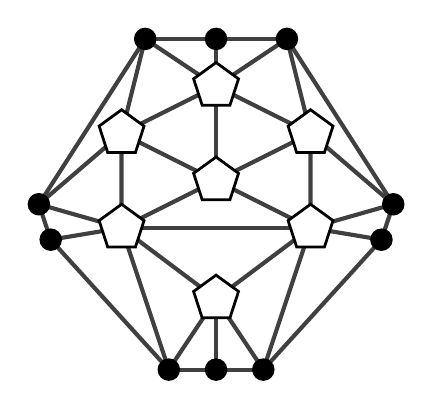
\begin{tikzpicture}[scale=0.6]
\VertexV[y=-1]{A}
	\VertexV[x=-2]{B}
	\VertexV[y=1]{C}
	\VertexV[x=2]{D}
	
	\VertexV[x=-2,y=-2]{E}
	\VertexV[x=2,y=-2]{F}
	\VertexV[y=-3.5]{G}
	
	\VertexI[x=-1.5,y=2]{V1}
	\VertexI[x=0,y=2]{V2}
	\VertexI[x=1.5,y=2]{V3}
	
	\VertexI[x=3.75,y=-1.5]{V4}
	\VertexI[x=3.5,y=-2.25]{V5}
	
	\VertexI[x=-1,y=-5]{V8}
	\VertexI[x=0,y=-5]{V7}
	\VertexI[x=1,y=-5]{V6}
	
	\VertexI[x=-3.75,y=-1.5]{V10}
	\VertexI[x=-3.5,y=-2.25]{V9}
	
	
	\Edge(A)(B)
	\Edge(A)(C)
	\Edge(A)(D)
	\Edge(B)(C)
	\Edge(C)(D)
	
	\Edge(E)(F)
	\Edge(F)(G)
	\Edge(G)(E)
	
	\Edge(E)(A)
	\Edge(F)(A)	
	\Edge(E)(B)
	\Edge(F)(D)
	
	
	\Edge(V1)(V2)
	\Edge(V2)(V3)
	\Edge(V3)(V4)
	\Edge(V4)(V5)
	\Edge(V5)(V6)
	\Edge(V6)(V7)
	\Edge(V7)(V8)
	\Edge(V8)(V9)
	\Edge(V9)(V10)
	\Edge(V10)(V1)
	
	\Edge(V1)(C)
	\Edge(V1)(B)
	\Edge(V2)(C)
	\Edge(V3)(C)
	\Edge(V3)(D)
	\Edge(V4)(D)
	\Edge(V4)(F)
	\Edge(V5)(F)
	\Edge(V6)(F)
	\Edge(V6)(G)
	\Edge(V7)(G)
	\Edge(V7)(G)
	\Edge(V8)(G)
	\Edge(V8)(E)
	\Edge(V9)(E)
	\Edge(V10)(E)
	\Edge(V10)(B)

\end{tikzpicture}
\end{subfigure}
\begin{subfigure}{0.1\textwidth}
\begin{tikzpicture}
\node[] at (0, 0) {$\implies$};
%\node[] at (0, 0) {};
\end{tikzpicture}
\end{subfigure}
\begin{subfigure}{0.4\textwidth}
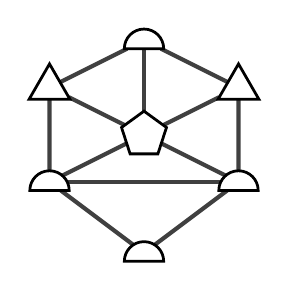
\begin{tikzpicture}[scale=0.6, yshift=5cm]
\VertexV[y=-1]{A}
	\VertexIII[x=-2]{B}
	\VertexII[y=1]{C}
	\VertexIII[x=2]{D}
	
	\VertexII[x=-2,y=-2]{E}
	\VertexII[x=2,y=-2]{F}
	\VertexII[y=-3.5]{G}
	
	
	
	\Edge(A)(B)
	\Edge(A)(C)
	\Edge(A)(D)
	\Edge(B)(C)
	\Edge(C)(D)
	
	\Edge(E)(F)
	\Edge(F)(G)
	\Edge(G)(E)
	
	\Edge(E)(A)
	\Edge(F)(A)	
	\Edge(E)(B)
	\Edge(F)(D)

\end{tikzpicture}
\end{subfigure}
\caption{An example of a non-$f$-colorable graph with a reducible configuration obtained from a cycle-canvas.}
\end{figure}

In fact, as \ref{fig:recursivereducibility} shows, this scenario can happen very easily when, 
for example, generating critical cycle-canvases, because it suffices to have a triangle with list 
sizes $2$ to make the graph non-$f$-colorable. The specific reducible configuration that appears 
in \ref{fig:recursivereducibility} is one of the small ones that we can check specifically before 
running Alon-Tarsi, but the more general scenario of having a reducible configuration plus a 
non-colorable subgraph does also often happen with larger reducible configurations and it is 
important that we deal with it automatically, using Alon-Tarsi to detect the reducible 
configuration.

What we do is the following: if Alon-Tarsi returns a negative answer to being applied to the 
entire graph, we try to find a \emph{minimal} non-colorable subgraph which is causing this 
negative answer (such 
as the triangle in \ref{fig:recursivereducibility}). We do that by arbitrarily removing vertices
and checking whether the graph is still non-$f$-colorable, and doing so until we have a graph
which becomes $f$-colorable when any vertex is removed. Then we remove subgraph $H$ (and reduce
the list sizes of vertices neighboring $H$ correspondingly, like when considering reducible 
configurations) and recursively apply the test to the remaining graph. We see that this works for
the graph in \ref{fig:recursivereducibility}: first, the triangle is removed and then the 
reducible configuration is identified. This recursive approach also handles more general cases
when there are multiple non-colorable subgraphs obstructing the colorability of the entire graphs.
Overall, the results of using this heuristic are very satisfactory. 

\begin{algorithm}[H]
\caption{Recursive Colorability Testing.}
\SetAlgoLined
\SetKwProg{Fn}{function}{}{end}
\SetKwComment{Comment}{/* }{ */}
\Fn{containsColorableSubgraph(G)}{
\If{$G$ is empty} {
	return false\;
}
\If{alonTarsi($G$)} {
	return true\;
}
$H \gets \text{minimalNonColorable}(G)$\;
return containsColorableSubgraph($\text{precolorSubgraph}(G,H)$)\;
\Comment*[r]{$\text{precolorSubgraph}(G,H)$ returns the graph $G$ removing the subgraph $H$ and decrementing the list sizes of the neighbors of vertices of $H$ appropiately.}
}
\Fn{minimalNonColorable(G)}{
	\For{$v \in V(G)$} {
		\If{not alonTarsi(removeVertex($G$,$v$))} {
			return minimalNonColorable(removeVertex($G$,$v$))\;
		}
	}
	return $G$\;
}


\end{algorithm}



\chapter{Approaches to the Two Precolored Triangles Theorem}

In this chapter we explain different approaches to proving Conjecture \ref{twotriangleconjecture}.

\section{Cycle-Canvas Strangulation}

We can generate all critical prism-canvases whose two triangles are at distance $d$ from critical
cycle-canvases with cycle size $2d+6$. Here is how:


\begin{proposition}
Let $G$ be a plane graph $(T_1 \cup T_2)$-critical with respect to some list assignment $L$, 
where $T_1$ and $T_2$ are two triangles 
and $P$ is a shortest path between them of length $d$. Let $G'$ be the graph
obtained by ``duplicating'' the $d+1$ vertices of path $P$, so that the edges of the path $P$ are
duplicated and the other neighbors of the duplicated vertices are now neighbors of the vertex
corresponding to the side of the path in which the neighbors were in (see Figure 
\ref{fig:strangulation}). Let $C$ be the corresponding cycle of length $2d+6$ that is newly formed
with the duplicated vertices and the vertices of the triangles. Then $G'$ is $C$-critical (with 
respect to the naturally corresponding list assignment $L'$).
\end{proposition}
\begin{proof}
By the Extension Lemma (\ref{extensionlemma}), $G$ is $(T_1 \cup T_2 \cup P)$-critical.
Now, the result follows by the Duplication Lemma (\ref{duplicationlemma}).
\end{proof}

\begin{figure}
\label{fig:strangulation}
\missingfigure{canvas strangulation}
\caption{Illustration of Canvas Strangulation}
\end{figure}

Now, we use this result in the backwards direction (as in Figure \ref{fig:strangulation}):
from critical cycle-canvases of cycle size $2d+6$, we generate candidates for critical 
prism-canvases by identifying $d+1$ consecutive vertices in the precolored cycle with the opposite
segment of $d+1$ consecutive vertices in the precolored cycle (it is useful to visualize 
the``inverted'' canvas, so that the precolored cycle is no longer the outer face but a cycle
bounding an interior face). Note that from each cycle-canvas there are $d+3$ ways to identify
the vertices. After criticality testing all candidates from all cycle-canvases of size $2d+6$, we
obtain all critical prism-canvases of distance $d$.

This can serve to get the list of
all critical prism-canvases with the triangles at a certain distance, which is useful
for a part of our plan and to experimentally determine the value of the right distance constant
in Conjecture \ref{twotriangleconjecture}.
However it is not useful, just by itself, to prove that there are no such critical prism-canvases
for large enough distances. 

\section{The Forbidden 3-3 Setting}

Recall Postle's approach: Postle, like Thomassen, works in a setting where the vertices of the 
outer face of the graphs are allowed to have lists of size $3$. 
For proving the Two Precolored Triangles Theorem, this is useful because a shortest path
between the triangles can be precolored to obtain a graph with two precolored paths
of length $1$ and vertices with list size at least $3$ in the outer face. The problem
is that there are infinitely many critical graphs in such a setting. The question is: can
we find some restriction on the list sizes so that:

\begin{enumerate}
	\item It is restrictive enough so that there are only finitely many $(P_1 \cup P_2)$-critical
	graphs, where $P_1, P_2$ are paths of length $1$ in the outer face, but
	\item It is not too restrictive, so it is useful and allows reductions like in the proof of
	Thomassen's Theorem.
\end{enumerate}

The setting we propose is: require vertices in the outer face to have list size at least $3$, and
also additionally require that no two adjacent non-precolored vertices have list size less than $4$. 
Note that in this setting, we cannot have the infinte amount of bellows that prevented
path-canvases with path length $2$ from being colorable, or the coloring harmonicas that prevented
canvases with a path of length $1$ and a path of length $0$ from being colorable.

In fact, this setting was first introduced in \cite{crossingsfarapart} to prove that there
are only finitely many $P$-critical graphs in this setting,
where $P$ is a path of length $2$, and as we will
see there are also only finitely many critical graphs for longer path lengths and for two 
paths of length $1$.

\begin{definition}
	We say that $(G, S, L)$ is a \emph{3-3-forbidden canvas} if $G$ is a connected plane graph
 with outer walk $C$, $S$ is a subgraph of $C$, and $L$ is a list assignment
  such that $|L(v)| \geq 5 \, \forall v \in V(G) \setminus V(C)$,
   $|L(v)| \geq 3 \, \forall v \in V(C) \setminus V(S)$ and for all $uv \in E(G)$ with 
   $u, v \not\in V(S)$ we have that $\max\{|L(u)|, |L(v)|\} \geq 4$. If $S$ is a path,
    we say $(G, S, L)$ is a \emph{3-3-forbidden wedge} (or just \emph{wedge} in this section). 
    If $S = P_1 \cup P_2$ with $P_1$, $P_2$ paths of length at most $1$, we say that $(G, S, L)$ is a
    \emph{3-3-forbidden biwedge}. We say that $(G, S, L)$ is critical if $G$ is $S$-critical
    with respect to $L$.
\end{definition}

Since in our program we do not store the list assignments for the graphs but we do store the 
prescribed list sizes for each vertex (that is, whether a vertex can have a list size of $3$ or
is forced to have $\geq 4$ colors), we will sometimes abuse terminology
 use the terms critical wedge and critical biwedge
to refer to those graphs with prescribed list sizes but not with a fixed list assignment.

\subsection{The Forbidden 3-3 Reduction}

Before we state the reduction that we can use in this setting, we need the following result:

\begin{proposition}
\ref{twocriticalwedgesprop}
There are only two critical 3-3-forbidden wedges with path length $2$:

\begin{enumerate}
	\item The three-vertex graph consisting of $P = p_0p_1p_2$ with an additional edge joining
	$p_0$ and $p_2$.
	\item The four vertex graph consisting of $P$ plus one vertex with list of size three joined
	to all three vertices of $P$.
\end{enumerate}

\end{proposition}

This is proven in \cite{crossingsfarapart} using the reduction we are about to describe,
but note that we can also prove it by generating critical wedges using the algorithm in 
Section \ref{sec:generationwedges} and seeing that it halts after generating only these two graphs.

\begin{definition}
We say that a 3-3-forbidden canvas $(G, S, L)$ is \emph{reducible} if the following holds:
\begin{enumerate}
	\item It is $2$-connected.
	\item The outer cycle has no chords.
	\item There is a precolored vertex $p_0 \in S$ so that the next four vertices 
	$v_1$, $v_2$, $v_3$, $v_4$ in clockwise order in the outer cycle are not in $S$. 
\end{enumerate}
\end{definition}

Let $(G, S, L)$ be a critical reducible 3-3-forbidden canvas, and consider the list sizes of
the vertices $v_1$, $v_2$, $v_3$, $v_4$ as in the definition of reducible. We are going to consider
different cases according to those list sizes, and in each case we will select a subset $X$ of those
vertices and a $L$-coloring on some of the vertices in $X$. 

\begin{figure}
\label{fig:reductioncases}
\centering
\missingfigure{reduction cases}
\caption{Illustration for the cases in the reduction}
\end{figure}

\begin{itemize}
	\item [X1] If $|L(v_2)| \geq 4$ and $|L(v_3)| \geq 4$, then $X = \{v_1\}$ and 
	$\phi(v_1) \in L(v_1) \setminus L(p_0)$ is chosen arbitrarily.
	\item [X2] If $|L(v_2)| \geq 4$ and $|L(v_3)| = 3$, then $X = \{v_1, v_2\}$ and $\phi$ is 
	chosen so that $\phi(v_2) \in L(v_2) \setminus L(v_3)$ and 
	$\phi(v_1) \in L(v_1) \setminus (L(p_0) \cup \{\phi(v_2)\})$.
	\item [X3] If $|L(v_2)| = 3$, and either $|L(v_4)| \neq 3$ or $|L(v_3)| \geq 5$, then 
	$X = \{v_2\}$ and $\phi(v_2) \in L(v_2)$ is chosen arbitrarily. 
	\item [X4] If $|L(v_2)| = 3$, $|L(v_3)| = 4$ and $|L(v_4)| = 3$, then:
	\begin{itemize}
		\item [X4a] If $v_1$, $v_2$ and $v_3$ do not have a common neighbor or 
		$|L(v_1)| \geq 5$, then $X = \{v_2, v_3\}$ and $\phi$ is chosen so that
		$\phi(v_3) \in L(v_3) \setminus L(v_4)$ and 
		$\phi(v_2) \in L(v_2) \setminus \{\phi(v_3)\}$.
		\item [X4b] If $v_1$, $v_2$ and $v_3$ have a common neighbor and $|L(v_1)|$ = 4, then
		$X = \{v_1, v_2, v_3\}$ and $\phi$ is chosen so that 
		$\phi(v_3) \in L(v_3) \setminus L(v_4)$, 
		$\phi(v_1) \in L(v_1) \setminus L(p_0)$ 
		and either at least one of $\phi(v_1)$ and $\phi(v_3)$
		does not belong to $L(v_2)$ or $\phi(v_1) = \phi(v_3)$. 
		The vertex $v_2$ is left uncolored.
	\end{itemize}
\end{itemize}

Let $G' = G \setminus X$ and let $L'$ be the list assignment obtained from $L$ by removing the colors 
of the vertices of $X$ according to $\phi$ from the lists of their neighbors (if a vertex of $X$ is not
colored according to $\phi$, we do not remove any colors for it). By the choice of $X$ and $\phi$,
any $L'$-coloring of $G'$ can be extended to an $L$-coloring of $G$, thus $G'$ is not $L'$-colorable.

This can imply one of these two options:

\begin{enumerate}
	
	\item $(G', S, L')$ contains a critical 3-3-forbidden canvas as a subgraph (and one which is 
	smaller than $(G, S, L)$.
	\item $(G', S, L')$ is not a 3-3-forbidden canvas.
\end{enumerate}

The second option can only happen if $G'$ contains two adjacent vertices with list size $3$. 
Let us call those vertices $u, v$. Because $G$ had no chords and because Lemma \ref{gluinglemma} and
Proposition \ref{twocriticalwedgesprop} applied to vertices of $G$ 
with two neighbors in $X$, we can conclude that $u$ and $v$ form a chord of the outer walk of $G'$.


\subsection{Plan for Critical Biwedges}

We will apply the above reduction to prove the following:

\begin{conjecture}
\label{biwedgeconjecture}
Let $(G, P_1 \cup P_2, f)$ be a tuple such that $G$ is a plane graph, $P_1$, $P_2$ are two length one 
paths in the outer walk of $G$, and $f$ is a list size assignment as in the definition of 3-3-forbidden
canvases. If there exists an $f$-list-assignment $L$ such that $(G, P_1 \cup P_2, L)$ is a critical
3-3-forbidden biwedge, then $(G, P_1 \cup P_2, f) \in \mathcal{S}$, where $\mathcal{S}$ is an explicit
finite set (to be determined computationally) such that all the members of $\mathcal{S}$ satisfy
$d(P_1, P_2) \leq 4$.
\end{conjecture}

In order to prove this, we do the following:

We can generate all critical biwedges with distance between paths $d$ by fusing all pairs of critical
wedges with path lengths $d+1$ or path lengths $d$ and $d+2$ as in figure \ref{fig:fusingwedges}
and testing criticality. 
By Lemma \ref{extensionlemma} applied to the shortest path between the two paths and Lemma 
\ref{gluinglemma}, all critical biwedges can be decomposed in this way. 

\begin{figure}
\label{fig:fusingwedges}
\missingfigure{fusing wedges}
\caption{Fusing wedges along the shortest path of the biwedge.}
\end{figure}

We let $\mathcal{S}$ be the set of critical biwedges with distance between paths
up to $4$ obtained by that procedure.

To prove the conjecture, assume for a contradiction that there is a critical biwedge $(G, P_1 \cup P_2,
f) \not\in \mathcal{S}$, and choose such a counterexample with the smallest $V(G)$. 

Assume $G$ has a chord or cutvertex. Then, by Lemma \ref{gluinglemma}, $G$ can be decomposed into
two smaller biwedges fused along the chord or cutvertex. We should verify computationally the following
statement:

\begin{proposition}
If any $B_1, B_2 \in \mathcal{S}$ are fused along one of their precolored paths to create a biwedge
$(G, P_1 \cup P_2, f)$ with $d(P_1, P_2) \geq 5$, then $(G, P_1 \cup P_2, f)$ is not critical.
\end{proposition}

So we conclude that $G$ can not have a chord or cutvertex. 

We must have $d(P_1, P_2) \geq 5$, since all critical biwedges with distance up to $4$ are in $S$.
Now, note that our biwedge is reducible. We apply the reduction. If $G$ contains as a 
subgraph a smaller critical biwedge, then that critical biwedge is in $\mathcal{S}$ 
and therefore has distance
at most $4$ between precolored paths, so $G$ shoud have distance at most $4$ between paths, 
contradiction.

Therefore we have that the resulting graph $G'$ after performing the reduction has a chord $uv$ with
two vertices of list size $3$. And $G'$ is not $L'$-colorable, so there exists a coloring of 
$P_1 \cup P_2$ that does not extend to $G'$, so $G'$ contains a subgraph $G''$ which is 
$(P_1 \cup P_2)$-critical with respect to $L'$. Now, $G''$ is not a critical biwedge
because of the $uv$ chord, but it by Lemma \ref{gluinglemma} it can be decomposed into two
critical smaller critical biwedges along the chord. Therefore, we must verify computationally
the following statement:

\begin{proposition}
If any $B_1, B_2 \in \mathcal{S}$ are fused along one of their precolored paths to create a 
triple $(G, P_1 \cup P_2, f)$
with \textbf{one chord between vertices with prescribed list sizes $3$ but no other adjacencies
between vertices with prescribed list size $3$}, then either $(G, P_1 \cup P_2, f)$ is not critical
\textbf{or} $d(P_1, P_2) \leq 4$. 
\end{proposition}
  
In order to reach a contradiction and conclude that such a counterexample must not exist. 

\subsection{Approach for Critical Triangle-Wedges} 

We can not use Postle's technique of precoloring a shortest path between the two
triangles to conclude the result for two triangles from the result for biwedges, because the
requirement that no two vertices adjacent vertices have list of size $3$ is too strong for
that.

Instead, what we can try is to use the reduction again. We generalize the two precolored triangles
setting as follows:

\begin{definition}
We say that $(G, S = P \cup T, L)$ is a \emph{3-3-forbidden triangle-wedge} if $G$ is a connected plane 
graph
 with outer walk $C$, $P$ is a  path of length $1$ of $C$, $T$ is a triangle bounding a face
 of $G$ (not necessarily incident with $C$)
 , and $L$ is a list assignment
  such that $|L(v)| \geq 5 \, \forall v \in V(G) \setminus (V(C) \cup V(T))$,
   $|L(v)| \geq 3 \, \forall v \in V(C) \setminus V(S)$ and for all $uv \in E(G)$ with 
   $u, v \not\in V(S)$ we have that $\max\{|L(u)|, |L(v)|\} \geq 4$. 
\end{definition}

Note that the critical prism-canvases can be retrieved from the critical 3-3-forbidden 
triangle-wedges by selecting those whose outer face is a triangle with list size $3$ in the outer
face. 

We can try a similar strategy as with the biwedges in order to prove that all the critical 
triangle-wedges belong to a critical set: construct all candidates in which the triangle is at a 
small distance from the outer face, and then apply the reduction to show that there are no critical
graphs with a larger distance.

But the problem is, here constructing all the graphs for which the triangle is at a small distance
from the outer face is much more complicated than for the biwedges.
It also requires larger critical wedges as building blocks, which we are less likely to be able to
be computed in reasonable time. In theory, this approach could be carried out with access to large
computational resources, but it seems like something smarter is needed. 



\chapter{Results and Further Study}

In this chapter we describe the computational results we got by executing our implementation
of the techniques described in the previous chapters, and briefly discuss next steps for
working on the 6-list-critical graphs on the torus problem.

\section{Computational Results}
\subsection{Generation of Cycle-Canvases}

\begin{table}[h]
\label{tab:cyclecanvases}
\centering
\begin{tabular}{l | l || l | l || l | l}
$\ell$ & \# & $\ell$ & \# & $\ell$ & \# \\
\hline
3 & 1 & 7  & 18    & 11 & 131221\\ 
4 & 1 & 8  & 145   & 12 & 1447449 \\
5 & 2 & 9  & 1260  & 13 & 16506284 \\ 
6 & 5 & 10 & 12518 & 14 & -- 
\end{tabular}
\caption{Number of critical cycle-canvases by cycle size}
\end{table}

In Table \ref{tab:cyclecanvases} we can see the number of cycle-canvases generated by our program
for sizes from $3$ to $13$. 
We see an exponential growth in the number of critical cycle-canvases, which is consistent with the
linear number of vertices bound of Theorem \ref{linearboundcycletheorem}. 
The base of the exponent appears to be approximately $10$.

Note that the number corresponds to \emph{candidates} for critical cycle-canvases (also including
the empty cycle-canvases, which are considered critical by our program for implementation ease), 
and the number of actual cycle-canvases could be slightly lower, especially in the higher cycle 
sizes. (This applies for all the tables in this chapter).

The generation of the critical cycle-canvases of cycle size $13$ takes around 10 hours in our 
computer. Our program uses too much memory for cycle-canvases of size $14$, because of the need to
store critical canvases in the queue and in the associative container used to eliminate duplicates.
We see the following possible improvements to ameliorate this:

\begin{itemize}
	\item Process the cycle-canvases in a depth-first rather than breadth-first way: that is,
	use a stack rather than a queue. Because the search space of critical cycle-canvases is 
	shallow with respect to the operation of adding a tripod, this will use less memory.
	\item Do not store the found cycle-canvases, just print them. This brings up the problem
	of how to handle duplicates: one possible way is to try to define a ``canonical'' sequence 		of tripod operations to generate any possible cycle-canvas, and only generate canvases
	through that canonical sequence of operations. This requires analyzing the symmetries of the
	graphs.
	\item Alternatively, compress the information of the generated graphs as much as possible
	while still retaining the ability to detect duplicates. Applying a compression hash function
	to the DFS transcript is the simplest example.

\end{itemize}

Also, we can also improve the time performance of the program via parallelization, since the program does criticality testing different graphs independently, and therefore can easily be 
parallelized.

We did in fact implement some of the proposals above, but it was not enough to achieve the 
generation of all critical cycle-canvases of cycle size $14$ in our computer. Nevertheless,
we believe that generating cycle-canvases of cycle size $14$ is feasible and can be achieved
by carefully optimizing the time and memory performance of our program or by running the program
in a computer with greater resources. However, the exponential growth in the number of critical 
cycle-canvases suggests that the practical limit might be $14$ or $15$. In particular, it is not 
feasible to generate all $~10^{10}$ critical cycle-canvases of cycle size $16$, which means that
if the appropiate constant in the Two Precolored Triangles Theorem is $5$, as we conjecture, we
will not be able to verify it by canvas strangulation.




\subsection{Generation of Prism-Canvases via Strangulation}



\begin{table}[h]
\label{tab:prismcanvases}
\centering
\begin{tabular}{l | l}
$d$ & \# \\
\hline
1 & 352 \\
2 & 1573\\ 
3 & 125 \\
\end{tabular}
\caption{Number of critical prism-canvases by distance between triangles}
\end{table}

Table \ref{tab:prismcanvases} shows the number of prism-canvases obtained by canvas strangulation
of cycle-canvases of cycle sizes $8$, $10$, $12$. The stark decline with prism-canvases at distance
$3$ gives us hopes that the number will reach $0$ by distance $5$ (or even $4$). 

Processing the critical cycle-canvases of cycle size $12$ to get the prism-canvases at distance $3$
takes about $30$ minutes in our computer, approximately the same time the cycle-canvas search 
program takes to generate the canvases of size $12$. The same optimizations, in particular
parallelization, can be applied to this program to make it faster. 

\subsection{Forbidden 3-3 Setting Approaches}

\begin{table}[h]
\label{tab:wedges}
\centering
\begin{tabular}{l | l}
$\ell$ & \# \\
\hline
1 & 1 \\
2 & 3 \\ 
3 & 22 \\
4 & 245 \\
5 & 3198 \\
6 & 44945 \\
\end{tabular}
\caption{Number of critical 3-3-forbidden wedges by path length}
\end{table}

\begin{table}[h]
\label{tab:biwedges}
\centering
\begin{tabular}{l | l | l}
$d$ & \# 2 Paths & \# Path \& Vertex \\
\hline
1 & 22   & 1\\
2 & 212  & 10\\ 
3 & 116  & 4 \\
4 & 14   & 0
\end{tabular}
\caption{Number of critical 3-3-forbidden biwedges by distance between precolored paths}
\end{table}

Table \ref{tab:wedges} shows the number of critical 3-3 forbidden wedges by path length up to
length $6$ and Table \ref{tab:biwedges} shows the number of biwedges (both those with two precolored
paths of length one and those with one path of length one and one path of length zero) generated
from those wedges by the distance between precolored paths up to distance $4$. We computationally performed the proof steps explained in Section . and therefore proved Conjecture ., which
we now restate here as two theorems. 

\todo{refs section and conjecture}

\begin{theorem}
There exist only finitely many 3-3-forbidden critical biwedges.
\end{theorem}

\begin{theorem}
Let $G$ be a plane graph with outer walk $C$, let $P_1, P_2$ be two paths of length $1$ in $C$, and let
$L$ be a list assignment for $G$. If all the following conditions are satisfied:

\begin{enumerate}
	\item $|L(v)| \geq 5 \, \forall v \in V(G) \setminus V(C)$.
	\item $|L(v)| \geq 3 \, \forall v \in V(C) \setminus (V(P_1) \cup V(P_2))$
	\item $P_1$, $P_2$ are $L$-colorable.
	\item There does not exist $uv \in E(G)$ with $|L(u)| = |L(v)| = 3$.
	\item $d(P_1, P_2) \geq 5$.
\end{enumerate}

then $G$ is $L$-colorable. 
\end{theorem}




\subsection{Criticality Strength Approaches}

\begin{table}[h]
\label{tab:strongwedges}
\centering
\begin{tabular}{l | l}
$\ell$ & \# \\
\hline
2 & 4 \\
3 & 269\\ 
4 & 31370 \\
\end{tabular}
\caption{Number of strong critical wedges by path length}
\end{table}

We can see in Table \cite{tab:strongwedges} that the number of strong critical wedges in the usual
canvas setting grows very fast, possibly exponentially with a base of around $100$. Therefore,
it is not feasible to reach wedges with length $9$, which are the ones we would need in the described 
approach. We tried other approaches using the
criticality strength ideas, but they suffer from similar combinatorial explosion issues. 

\section{Conclusions and Further Study}

We hope that the work done in this thesis can serve as a first step in the quest for finding the
set of 6-list-critical graphs on the torus. Based on the results we have gotten above and what 
we have studied about the problem, we outline some possible next steps to be taken:

\begin{itemize}
	\item Implement the corresponding optimizations to the critical cycle-canvas search and
	canvas strangulation programs in order to obtain the list of critical cycle-canvases with
	cycle size $14$ and the list of critical prism-canvases with triangle distance $4$. 
	We discussed the details of what those optimizations could be in the previous 
	section.
	\item Try to prove the Two Precolored Triangles Theorem with the tightest bound. 
	This is the main obstacle we have faced for our plan. 
	Our approaches have not been successful: the 3-3-forbidden
	setting worked well for the biwedges but it is not conceptually clear how to extend
	it to the precolored triangle setting, and the approaches based on generating only strong
	critical graphs have computational issues because there are too many graphs. Perhaps
	more work and more complex strategies can make these approaches successful, or
	perhaps new ideas are needed here.
	\item Implement gluing of prism-canvases along the precolored triangles to generate
	new candidates for critical prism-canvases with a separating triangle. This may allow
	us to get some critical prism-canvases with higher distances (if those exist) without
	having to strangulate cycle-canvases of large cycle size.
	\item Implement resconstruction of critical $6$-list-critical graphs on the torus
	from critical cycle-canvases and prism-canvases. This will allow us to see if we have
	found any counterexample to Conjecture \ref{torusconjecture}, and will at least allow
	us to prove a weaker result about the colorability of graphs on the torus with bounded
	distance between non-contractible triangles even if we do not prove the Two Precolored
	Triangles Theorem with a good bound. 
	\item Think about what to do for graphs on the torus without non-contractible triangles.
	
\end{itemize}








\newpage

\todo{fix bibliography (not arxiv version, extraneous urls, etc)}

\printbibliography
\end{document}


